\documentclass[a4paper, 14pt, oneside]{Thesis}
\usepackage[normalem]{ulem}  % normalem keeps \emph as italics instead of underline
\usepackage[square, numbers, comma, sort&compress]{natbib}  % Use the "Natbib" style for the references in the Bibliography
\usepackage{verbatim}
\usepackage{iftex}
\ifPDFTeX
  \usepackage{pslatex} %To set the font as Times New Roman (pdfLaTeX, e.g. Overleaf)
\else
  \usepackage{newtxtext,newtxmath} % Times equivalent for XeLaTeX/LuaLaTeX
\fi
\usepackage{amsbsy}
\usepackage{amsfonts}
\usepackage{graphicx}
\usepackage{dcolumn}
\usepackage{amsmath}
\usepackage{latexsym}
\usepackage{amssymb}
\usepackage{epsfig}
\usepackage{epsfig,graphics}
\usepackage{subfigure}
\usepackage{tikz}
\usetikzlibrary{positioning,arrows.meta,fit,backgrounds,shapes.geometric,calc}
\usepackage{pgfplots}
\pgfplotsset{compat=1.17}
\usepackage{float}
\usepackage{algorithm}
\usepackage{algpseudocode}
\usepackage{placeins}  % For FloatBarrier
\usepackage{tabularx}
\usepackage{array}
\usepackage{multirow}

%To have 1. instead of [1] in the bibliographic entry
\makeatletter
\renewcommand\@biblabel[1]{#1.}
\makeatother

% To remove hyphenation
\tolerance=1
\emergencystretch=\maxdimen
\hyphenpenalty=10000
\hbadness=10000
%
%----To make sure the page numbers are in the top middle of each page.
\fancypagestyle{Thesis}{
\fancyhf{}
\fancyhead[C]{\thepage}
\pagestyle{fancy}
}
%----------------------------------------------------------------------
%% Project-specific macros
\algrenewcommand\algorithmicrequire{\textbf{Input:}}
\algrenewcommand\algorithmicensure{\textbf{Output:}}
\makeatletter
\algrenewcommand\ALG@beginalgorithmic{\small}   % keep long algorithms within a page at 14pt
\makeatother
\definecolor{phaseone}{gray}{0.90}
\definecolor{seriesA}{HTML}{2A78D6}   % blue
\definecolor{seriesB}{HTML}{EB6834}   % orange
\definecolor{seriesC}{HTML}{1BAF7A}   % aqua
\definecolor{neutralbar}{HTML}{9A9994}
\newcommand{\fillin}[1]{\textcolor{red}{[#1]}}   % values still to be supplied
\newcommand{\QtoA}{Q$\rightarrow$A}
\newcommand{\QAtoR}{QA$\rightarrow$R}
\newcommand{\QtoAR}{Q$\rightarrow$AR}
\newcommand{\code}[1]{\texttt{#1}}
\newcolumntype{L}{>{\raggedright\arraybackslash}X}
%% image with automatic placeholder box when the file is missing
\newcommand{\figimg}[2]{%
  \IfFileExists{#2}{\includegraphics[width=#1]{#2}}{%
    \fbox{\parbox[c][5.5cm][c]{\dimexpr#1-2\fboxsep-2\fboxrule\relax}{\centering\small
      \textcolor{red}{Place image here:}\\[2pt]\texttt{\detokenize{#2}}}}}}
\renewcommand\appendixname{APPENDIX}
%% ------------------------s----------------------------------------
% Some new environments for the paper
%
\newtheorem{dfn}{Definition}[section]
\newtheorem{prop}[dfn]{Proposition}
\newtheorem{lem}[dfn]{Lemma}
\newtheorem{thm}[dfn]{Theorem}
\newtheorem{cor}[dfn]{Corollary}
\newtheorem{clm}[dfn]{Claim}
\newtheorem{fact}[dfn]{Fact}
%
%\newcommand{\RightBox}{\begin{flushright} $\Box$ \end{flushright}}
\newcommand{\RightBox}{{\phantom{a}}\hfill $\Box$ \\}
%\newenvironment{proof}{{\bf Proof:~}}{\RightBox}
\newenvironment{prf}{{\bf Proof~Idea:~}}{\RightBox}
%\newcommand{\claim}[1]{{\bf Claim #1:~}}
%
\newcommand{\Dfn}[1]{Definition \ref{dfn:#1}}
\newcommand{\Prop}[1]{Proposition \ref{prop:#1}}
\newcommand{\Lem}[1]{Lemma \ref{lem:#1}}
\newcommand{\Thm}[1]{Theorem \ref{thm:#1}}
\newcommand{\Cor}[1]{Corollary \ref{cor:#1}}

%Action-indexed diamond modality
\newcommand{\Adiam}[1]{\mbox{$\langle #1 \rangle$}}
\newcommand{\diamin}{\Diamond\kern-0.5em{\raisebox{.25ex}{\rm -}}\kern0.175em}
\newcommand{\until}{\mbox{\large\bf U}}
\newcommand{\since}{\mbox{\large\bf S}}
\newcommand{\nxt}{\mbox{$\bigcirc$}}
\newcommand{\nxtdot}{\displaystyle \bigodot}
\newcommand{\past}{\diamin}
\newcommand{\ifpast}{\mbox{$\boxminus$}}
\newcommand{\now}{\mbox{$\langle now \rangle$}}
\newcommand{\Now}{\mbox{$[now]$}}
\newcommand{\pres}{\mbox{$\rangle \langle$}}
\newcommand{\snd}{\mbox{\large\bf s}}
\newcommand{\rec}{\mbox{\large\bf r}}
\newcommand{\nc}{\mathbf{no\_comm}}

%Propositional connectives
%\newcommand{\implies}{{\raisebox{.20ex}{$\scriptstyle ~\supset~$}}}
\newcommand{\Not}{\mbox{$\lnot$}}
\newcommand{\xor}{\oplus}
\newcommand{\True}{\mathit{True}}
\newcommand{\False}{\mathit{False}}
\newcommand{\Imply}{\supset}
%Large symbols
\newcommand{\andover}{\displaystyle \bigwedge}
\newcommand{\orover}{\displaystyle \bigvee}
\newcommand{\capover}{\displaystyle \bigcap}
\newcommand{\cupover}{\displaystyle \bigcup}
\newcommand{\piover}{\displaystyle \Pi}
\newcommand{\ohat}[1]{\widehat{#1}}
\newcommand{\otilde}[1]{\widetilde{#1}}
\newcommand{\obar}[1]{\overline{#1}}
\newcommand{\Sigtil}{\mbox{$\otilde{\Sigma}$}}
\newcommand{\DA}{\mbox{$\Sigtil~=~(\Sigma_1, \dots, \Sigma_n)$}}

%Useful symbols
\newcommand{\derives}{\vdash}
\newcommand{\defn}{\mbox{$~\stackrel{\rm def}{=}~$}}
\newcommand{\qneq}{\mbox{$~\stackrel{\rm ?}{=}~$}}
\newcommand{\eqv}{\approx}
\newcommand{\hash}{\sharp}
\newcommand{\restr}{\lceil}
%\newcommand{\bot}{\bottom}
\newcommand{\nat}{{\bf N}}
\newcommand{\pfin}[1]{\mbox{$\wp_{fin}(#1)$}}
%\newcommand{\mod}[1]{\mbox{$|#1|$}}
\newcommand{\memb}[2]{\mbox{${#1} \in {#2}$}}
\newcommand{\E}{\mathbf{E}}



%Some roman words in math mode
\newcommand{\Iff}{\mbox{~iff~}}
\newcommand{\Where}{\mbox{~where~}}
%\newcommand{\And}{\mbox{~and~}}
\newcommand{\Implies}{\mbox{~implies~}}

%Relations

% structures
\newcommand{\Sigstr}{\mbox{$\Sigma^*$}}
\newcommand{\TS}{\mbox{$TS = (Q,\to)$}}  %generates TS=(Q,->)
\newcommand{\TSP}{\mbox{$TS = (Q,\To)$}}         %generates TS=(Q,=>)
\newcommand{\TSi}{\mbox{$TS_i = (Q_i,\to_i)$}}           
\newcommand{\TSE}{\mbox{$TS_{ES}$}}
\newcommand{\TSN}{\mbox{$TS_{\cal N}$}}
\newcommand{\ES}{\mbox{$ES = (E,\leq,\#)$}}       %generates ES=(E,<=,#)
\newcommand{\LES}{\mbox{$ES = (E,\leq,\#,\phi)$}} %generates ES=(E,<=,#,phi)
\newcommand{\Tmdl}{\mbox{$M = (TS,V)$}}          %generates M = (TS,V)
\newcommand{\cfin}[1]{\mbox{$C_{#1}$}}           %finite configurations of
\newcommand{\fincon}[1]{\mbox{$C_{#1}^{fin}$}}  %finite configurations

% classes
\newcommand{\mdl}[1]{\mbox{${\cal M}_{#1}$}}%generates script M with subscript
\newcommand{\dmodels}{\mbox{$\models_{Det}~$}}

% For transitions steps
\newcommand{\step}[1]{\mbox{$\stackrel{#1}{\to}$}}
\newcommand{\Funnyto}{\rightsquigarrow}
\newcommand{\longstep}[1]{\mbox{$\stackrel{#1}{\longrightarrow}$}}
\newcommand{\emptystep}{\step{\emptyset}}
\newcommand{\reach}[1]{\mbox{${\cal R}(#1)$}}
\newcommand{\reachin}[2]{\mbox{${\cal R}_{#1}(#2)$}}

% For a "double-lined" transition relation
\newcommand{\To}{\Rightarrow}
\newcommand{\From}{\Leftarrow}
\newcommand{\Step}[1]{\mbox{$\stackrel{#1}{\To}$}}
\newcommand{\Longstep}[1]{\mbox{$\stackrel{#1}{\Longrightarrow}$}}
\newcommand{\Longlongstep}[1]{\mbox{$\stackrel{#1}{\Longlongrightarrow}$}}
\newcommand{\Emptystep}{\Step{\emptyset}}

% Net theory
\newcommand{\presca}[1]{\mbox{${ }^{\bullet}#1$}}
\newcommand{\postsca}[1]{\mbox{$#1 \, { }^{\bullet}$}}%

%The built in downarrow generates too much space after it
%\newcommand{\down}{\mbox{$\downarrow \!$}}
\newcommand{\down}{\mbox{$\downarrow$}}
\newcommand{\up}{\mbox{$\uparrow \!$}}
\newcommand{\ldot}{{\rm <}\kern-0.37em{\raisebox{.25ex}{\bf .}}\kern0.375em}

%Trace theory
\newcommand{\edoti}{\mbox{$\doteq_I$}}
\newcommand{\eqi}{\mbox{$=_I$}}
\newcommand{\edotk}{\mbox{$\doteq_k$}}
\newcommand{\eqk}{\mbox{$=_k$}}

\newcommand{\calL}{\mathcal{L}}
\newcommand{\calB}{\mathcal{B}}
\newcommand{\posetlang}[1]{\mbox{${\calL}^{po}(#1)$}}%poset language of an SCA
\newcommand{\bddlang}[2]{\mbox{${{\calL}^{#1}}(#2)$}} %bounded buffer language

\newcommand{\calS}{\mathcal{S}}
\newcommand{\calA}{\mathcal{A}}
\newcommand{\calC}{\mathcal{C}}
\newcommand{\calE}{\mathcal{E}}
\newcommand{\calG}{\mathcal{G}}



\newcommand{\calQ}{\mathcal{Q}}
\newcommand{\calD}{\mathcal{D}}
\newcommand{\calCN}{\mathcal{CN}}
\newcommand{\calI}{\mathcal{I}}
\newcommand{\calF}{\mathcal{F}}
\newcommand{\calM}{\mathcal{M}}

\begin{document}

\frontmatter	  % Begin Roman style (i, ii, iii, iv...) page numbering


%  Title Page

\title{EXPLAINABLE VISUAL COMMONSENSE REASONING FOR SOCIAL INTERACTIONS}
\authors  {{ VIJAY SHERWIN G \hspace{0.4in} 3122235001158\\ \vspace{0.1in}}
{ UDHAYA SAKTHI K \hspace{0.4in} 3122235001152\\ \vspace{0.1in}}
{ THIRILOGSHA S S \hspace{0.4in} 3122235001147\\ \vspace{0.1in}}
}
\addresses  {\\\Computer Science \& Engineering\\}
\date       {\large {November 2026}}

\maketitle
%% ----------------------------------------------------------------

\setstretch{1.3}
\fancyhead{}  % Clears all page headers and footers
\rhead{\thepage}  % Sets the right side header to show the page number
\lhead{}  % Clears the left side page header

\pagestyle{fancy}  % Finally, use the "fancy" page style to implement the FancyHdr headers


\Declaration{
%
\quad Certified that this project report titled \textbf{``EXPLAINABLE VISUAL COMMONSENSE REASONING FOR SOCIAL INTERACTIONS''} is the \textit{bonafide} work of \textbf{VIJAY SHERWIN G (3122235001158)}, \textbf{UDHAYA SAKTHI K (3122235001152)} and \textbf{THIRILOGSHA S S (3122235001147)} who carried out the project work under my supervision.
\\
Certified further that to the best of my knowledge the work reported herein does not form part of any other thesis or dissertation on the basis of which a degree or award was conferred on an earlier occasion on this or any other candidate. \\

\begin{flushleft}
\begin{minipage}[t]{0.45\linewidth}
    \textbf{Dr. T.T. MIRNALINEE}\\
    \textbf{HEAD OF THE DEPARTMENT}\\
    Professor\\
    Department of CSE\\
    SSN College of Engineering\\[6pt]
    Kalavakkam - 603 110
\end{minipage}
\hfill
\begin{minipage}[t]{0.45\linewidth}
    \textbf{Dr. M. SARITHA}\\
    \textbf{SUPERVISOR}\\
    Assistant Professor\\
    Department of CSE\\
    SSN College of Engineering\\[6pt]
    Kalavakkam - 603 110
\end{minipage}
\end{flushleft}


\medskip
Submitted for project viva-voce examination held on\ldots\ldots\ldots\ldots
\\
\\
\\
{\bf EXTERNAL EXAMINER}\hfill
{\bf INTERNAL EXAMINER}
}
\clearpage

%% ----------------------------------------------------------------
% Acknowledgements

\acknowledgements{
We thank GOD, the almighty for giving us the strength and knowledge to do this project.

We would like to express our deep sense of gratitude to our guide \textbf{Dr. M. SARITHA}, Assistant Professor, Department of Computer Science and Engineering, for the valuable advice and suggestions as well as the continued guidance, patience and support that helped us to shape and refine our work.

Our sincere thanks to \textbf{Dr. T.T. MIRNALINEE}, Professor and Head of the Department of Computer Science and Engineering, for the words of advice and encouragement. We would like to thank our project panel members for their valuable suggestions throughout this project.

We also express our appreciation to \textbf{Dr. S. RADHA}, Principal, for all the help rendered during this course of study.

We would like to extend our sincere thanks to all the teaching and non-teaching staff of our department who have contributed directly and indirectly during the course of our project work.
Finally, we would like to thank our parents and friends for their patience, cooperation and moral support throughout our life.
\newline
\newline
\newline
\newline
{\bf VIJAY SHERWIN G}\hfill
{\bf UDHAYA SAKTHI K}\hfill
{\bf THIRILOGSHA S S}
\clearpage  % Acknowledgements ended, start a new page

\addtotoc{ABSTRACT} % Add the "Abstract" page entry to the Contents
\abstract{ \begin{spacing}{1.8}
The activity, relationship and intention behind a social interaction in an image are rarely visible directly; they must be inferred from visual cues together with everyday commonsense knowledge. This project builds an explainable Visual Commonsense Reasoning system that predicts these three aspects and supports every prediction with evidence that a user can inspect. Phase I, presented in this report, builds the prediction pipeline: the input is standardised using OpenCV, a lightweight vision-language model (SmolVLM) describes the people, actions and setting, ConceptNet supplies related commonsense knowledge, and a log-linear fusion stage produces the three predictions with confidence scores, ranked alternatives and a textual explanation. SmolVLM is also fine-tuned on the VCR dataset with LoRA; the selected checkpoint (epoch 11 of 20) raises \QtoAR{} accuracy on held-out VCR questions from 15.3\% to 32.7\%. The pipeline is exposed through a FastAPI--React interface and passes all 23 automated tests. Phase II will verify the explanations through visual attribution, cross-modal consistency and faithfulness evaluation, and present them in an explainability dashboard.
\end{spacing}
}
\clearpage

\pagestyle{plain}  %The page style headers have been "empty" all this time, now use the "fancy" headers as defined before to bring them back

%% ----------------------------------------------------------------
\lhead{\emph{Contents}}  % Set the left side page header to "Contents"

\tableofcontents % Write out the Table of Contents


%% ----------------------------------------------------------------
\lhead{\emph{List of Tables}}  % Set the left side page header to "List of Tables"
\listoftables

%% ----------------------------------------------------------------
\lhead{\emph{List of Figures}}  % Set the left side page header to "List if Figures"
\listoffigures  % Write out the List of Figures


\mainmatter	  % Begin normal, numeric (1,2,3...) page numbering
\pagestyle{myheadings}  % Return the page headers back to the "fancy" style

\begin{spacing}{1.5}
% Chapter 1

\chapter{INTRODUCTION} % Write in your own chapter title
\label{ch:intro}

Visual understanding has progressed from object recognition to higher-level reasoning about actions, relationships, context and human intention. Social interactions are particularly challenging because their interpretation depends on several people at once, on their posture and gestures, on the objects they use, on their spatial arrangement and on the wider context. Visual Commonsense Reasoning (VCR) extends conventional recognition by requiring a model to infer information that is not explicitly visible in an image~\cite{zellers2019vcr}.

This report presents the first phase of a system that performs such reasoning for social interactions and exposes the evidence behind each of its conclusions. The input is standardised using OpenCV, a lightweight vision-language model (SmolVLM) identifies the people, actions, gestures and setting of the scene, ConceptNet supplies everyday commonsense knowledge related to these concepts, and a reasoning module fuses the evidence to predict the activity, the relationship and the intention of the interaction. Each prediction is returned with a confidence value, ranked alternatives, supporting evidence and a textual explanation. SmolVLM is also fine-tuned on the VCR dataset with LoRA so that it reasons more reliably about people.

\section{MOTIVATION}

A photograph of two people shaking hands may show a business deal, a greeting between friends, a sporting gesture or a reconciliation after an argument. The pixels are much the same in each case; what differs is the context and the commonsense knowledge a person brings to the scene. Humans make these inferences effortlessly, but automated systems that make them are increasingly used in settings where the inference matters: assistive tools that describe scenes to visually impaired users, social robots that must decide how to approach people, and tools that summarise or moderate visual media.

Two problems limit the use of current models in such settings. The first is \textbf{opacity}. High-accuracy VCR models select an answer from a set of options but do not show which visual cues or which pieces of world knowledge led to the choice. Large generative vision-language models do produce explanations, but these explanations are not guaranteed to reflect the evidence the model actually used, and they can describe details that are not present in the image. The second is \textbf{cost}. The strongest multimodal models have tens of billions of parameters and require data-centre hardware, which rules them out for on-device, privacy-preserving or low-cost deployment.

This project is motivated by the need for a system that is both \emph{lightweight} and \emph{inspectable}: it should run on modest hardware, and every prediction about a social interaction should come with structured evidence -- the visual concepts detected, the commonsense facts used, the probabilities from each source and the alternatives that were considered -- that a user can check.

\section{BACKGROUND}

\subsection{Visual Commonsense Reasoning}

The VCR task, introduced by Zellers et al.~\cite{zellers2019vcr}, poses a multiple-choice question about an image taken from a movie scene. The people and objects in the image are referred to by tags such as \emph{person1} and \emph{person2}. A model must solve two sub-tasks: \QtoA, choosing the correct answer from four options, and \QAtoR, choosing the rationale that justifies the correct answer from four options. The joint metric \QtoAR{} counts a question as correct only when both the answer and the rationale are correct. With four options each, chance accuracy is 25\% for \QtoA{} and \QAtoR{} and 6.25\% for \QtoAR.

\subsection{Vision-Language Models}

A vision-language model (VLM) couples an image encoder with a language model so that it can describe images and answer questions about them. Modern VLMs encode the image into a sequence of visual tokens, project them into the embedding space of a pre-trained language model, and generate text autoregressively~\cite{liu2023llava,li2023blip2}. SmolVLM~\cite{marafioti2025smolvlm} is a family of compact VLMs designed for efficient inference. The variant used in this project, \code{SmolVLM-Instruct}, has about 2.2 billion parameters and combines a SigLIP vision encoder~\cite{zhai2023siglip} with a small language model through a connector that compresses the visual tokens.

\subsection{Commonsense Knowledge Graphs}

ConceptNet~\cite{speer2017conceptnet} is a multilingual knowledge graph of everyday knowledge. Its nodes are words and phrases (for example \emph{concert}, \emph{sing}, \emph{stage}) and its edges are labelled relations such as \emph{RelatedTo}, \emph{IsA}, \emph{UsedFor}, \emph{AtLocation}, \emph{CapableOf}, \emph{Antonym} and \emph{DistinctFrom}, each with a confidence weight. Because each edge is a readable statement (``a performer is typically found at a stage''), ConceptNet is well suited to producing evidence that a human can inspect.

\subsection{Parameter-Efficient Fine-Tuning}

Fine-tuning all the weights of a multi-billion-parameter model is expensive. Low-Rank Adaptation (LoRA)~\cite{hu2022lora} freezes the pre-trained weight matrix $W_0 \in \mathbb{R}^{d \times k}$ and learns a low-rank update:
\begin{equation}
  h = W_0 x + \frac{\alpha}{r} B A x, \qquad
  B \in \mathbb{R}^{d \times r},\; A \in \mathbb{R}^{r \times k},\; r \ll \min(d,k)
  \label{eq:lora}
\end{equation}
where $r$ is the rank and $\alpha$ a scaling factor. Only $A$ and $B$ are trained, so the number of trainable parameters and the optimiser memory are a small fraction of full fine-tuning, and after training $BA$ can be merged into $W_0$ so that inference is no slower than with the base model.

\subsection{Explainability and Faithfulness}

An explanation is \emph{plausible} if it convinces a human and \emph{faithful} if it reflects the reasoning the model actually performed. Visual explanation methods such as Grad-CAM~\cite{selvaraju2017gradcam} highlight the image regions that most influence a prediction. Their faithfulness can be measured with the Insertion--Deletion metric~\cite{petsiuk2018rise}, which tracks how the model's confidence changes as the highlighted pixels are added or removed, and with the Pointing Game~\cite{zhang2018excitation}, which checks whether the most salient point falls inside the relevant object. Textual explanations can be compared with visual explanations to measure cross-modal consistency~\cite{zhang2024crossmodal,parcalabescu2025faithfulness}. These methods form the basis of Phase II of this project.

\section{PROBLEM DEFINITION}

A social interaction may be visually ambiguous even when the people and objects in the scene are detected correctly. A system may recognise two people and their gestures but still need commonsense knowledge to distinguish between possible activities, or to infer the relationship and intention behind the interaction. The problem addressed in this project is therefore:

\begin{quote}
\itshape Given a static image, video frame, or live-camera frame containing zero or more people, develop a lightweight system that identifies the visual concepts in the scene, enriches them with commonsense knowledge, and predicts the activity, relationship, and intention of a social interaction with interpretable evidence.
\end{quote}

\subsection{Inputs}
The system accepts a static image, supplied as a file path, a URL, a NumPy array or a PIL image, as well as sampled frames from a video file and frames from a live camera. Along with the visual input, the user may ask an optional free-form question about the scene and may also supply multiple-choice answer options for that question.

\subsection{Outputs}
The principal output is a structured prediction of the activity, relationship and intention of the interaction. Each of the three predictions carries a label, a confidence value and a ranked list of alternative labels, and every alternative records its VLM probability, commonsense probability and draft-match value. The prediction is accompanied by its supporting evidence and a generated textual explanation. The intermediate results are returned as well: the visual concepts and draft reasoning produced by the VLM, the ConceptNet facts and label-support scores, and the processing time of each module.

\subsection{Constraints}
The system is built around lightweight multimodal models so that it can run on modest hardware. The ConceptNet integration uses a local SQLite database for reproducible offline operation and can fall back to other configured backends. The label space used for reasoning is configurable through \path{configs/taxonomy.yaml}.

\subsection{Scope of Phase I}
The complete framework follows the workflow
\begin{center}
\small\textbf{Input $\rightarrow$ Preprocessing $\rightarrow$ VLM $\rightarrow$ Commonsense $\rightarrow$ Reasoning $\rightarrow$ Explanation $\rightarrow$ Consistency $\rightarrow$ Evaluation $\rightarrow$ Dashboard}
\end{center}
Phase I, reported here, covers the first four modules -- Input and Preprocessing, the Small Vision-Language Model, ConceptNet Commonsense Enrichment and Social Interaction Reasoning -- together with the offline fine-tuning of SmolVLM on VCR. Its deliverable is a working pipeline that takes visual input and produces a social-interaction prediction with a draft explanation. Phase II adds the textual and visual explanation paths, cross-modal consistency analysis, explainability evaluation and the final explainability dashboard.

\section{ORGANIZATION OF THE REPORT}

This project report is divided into chapters, each describing a significant component of the work performed. Chapter~\ref{ch:intro} introduces the project by explaining the motivation, the background of the study and the problem statement. Chapter~\ref{ch:lit} surveys the literature on visual commonsense reasoning, vision-language models, knowledge-augmented reasoning, social relation recognition and explainability, identifies the gaps this project addresses and states the research objectives.

Chapter~\ref{ch:method} explains the proposed methodology in detail: the overall architecture, each Phase I module with its algorithm, the LoRA fine-tuning procedure and the integration of the modules. Chapter~\ref{ch:results} describes the datasets, the hardware and software ecosystem and the experiments conducted, and analyses the results.

Chapter~\ref{ch:impact} discusses the social impact and sustainability of the proposed system. Chapter~\ref{ch:conclusion} concludes the report and outlines the work planned for Phase II. The appendices list the configuration parameters and the API endpoints of the implementation.
 % INTRODUCTION
% Chapter 2

\chapter{LITERATURE SURVEY} % Write in your own chapter title
\label{ch:lit}

This chapter reviews work in five areas that bear on the problem: models and datasets for visual commonsense reasoning, pre-trained and instruction-tuned vision-language models, reasoning with external knowledge, recognition of social relations, and the explanation and evaluation of multimodal models.

\section{PAPERS RELATED TO THE PROBLEM IDENTIFIED}

\subsection{Recognition to Cognition Network (R2C)}
Zellers et al.~\cite{zellers2019vcr} introduced the VCR dataset and the Recognition-to-Cognition network (R2C). R2C grounds the words of the question and the candidate responses in detected object regions, contextualises the response with respect to the question and the image, and reasons over the result to score each option. The dataset was constructed with \emph{Adversarial Matching}, which reuses correct answers from other questions as distractors so that the wrong options are fluent and relevant. The paper showed a large gap between the best model and human performance, establishing VCR as a benchmark for cognition-level understanding.

\subsection{Tags and Attributes for VCR (TAB-VCR)}
Lin et al.~\cite{lin2019tabvcr} proposed TAB-VCR, a simpler baseline that attaches attributes to the detected objects and adds new tags for objects that are mentioned in the text but not tagged in the image. The improved visual grounding gave higher accuracy than R2C with fewer parameters, showing that better grounding of text in image regions matters more than model complexity.

\subsection{Heterogeneous Graph Learning (HGL)}
Yu et al.~\cite{yu2019hgl} proposed Heterogeneous Graph Learning, which builds a vision-to-answer graph and a question-to-answer graph and uses a contextual voting module to exploit long-range visual context. It models the relations between visual and linguistic elements explicitly, but its reasoning remains internal to the network.

\subsection{VisualCOMET}
Park et al.~\cite{park2020visualcomet} introduced VisualCOMET, a dataset of more than a million textual commonsense inferences about still images, describing what may have happened before, what may happen next and the intents of the people in the scene. It frames visual commonsense as the generation of inferences rather than the selection of options, which is closer to the explanations this project produces.

\subsection{Pre-trained Vision-Language Transformers}
ViLBERT~\cite{lu2019vilbert} extended BERT to a two-stream architecture in which visual and textual streams interact through co-attentional transformer layers, pre-trained on image--caption pairs and transferred to tasks including VCR. VL-BERT~\cite{su2020vlbert} used a single-stream transformer over both modalities, and UNITER~\cite{chen2020uniter} learned a universal image--text representation from several large datasets with word--region alignment objectives, reaching state-of-the-art VCR accuracy at the time. MERLOT~\cite{zellers2021merlot} learned multimodal script knowledge from millions of YouTube videos and their transcripts, and transferred well to VCR. These models raised VCR accuracy considerably, but they are discriminative classifiers: they score given options and provide no explanation of their own beyond attention weights, which are not reliable indicators of the evidence used.

\subsection{Generative Vision-Language Models}
CLIP~\cite{radford2021clip} trained image and text encoders contrastively on 400 million image--text pairs, enabling zero-shot recognition from natural-language labels. BLIP-2~\cite{li2023blip2} connected a frozen image encoder to a frozen large language model through a lightweight Querying Transformer, and LLaVA~\cite{liu2023llava} connected a CLIP encoder to an instruction-tuned language model and trained it on machine-generated visual instruction data. These generative VLMs answer open questions and produce fluent free-form explanations, but the largest of them are expensive to run and their explanations can include details that are not present in the image.

\subsection{SmolVLM: Compact Vision-Language Models}
SmolVLM~\cite{marafioti2025smolvlm} targets the opposite end of the design space: compact models with aggressive visual-token compression, intended for on-device and low-memory inference. Its vision encoder is based on SigLIP~\cite{zhai2023siglip}. SmolVLM makes a VLM practical on a laptop, which is why it is used in this project, but on its own it is not adapted to commonsense reasoning about people.

\subsection{Knowledge-Augmented Visual Reasoning}
ConceptNet 5.5~\cite{speer2017conceptnet} provides a large graph of general knowledge whose edges are readable statements. OK-VQA~\cite{marino2019okvqa} is a VQA benchmark whose questions cannot be answered from the image alone and require external knowledge. KRISP~\cite{marino2021krisp} combined the implicit knowledge of a pre-trained transformer with symbolic knowledge from graphs, including ConceptNet, through a graph network, and showed that both kinds of knowledge contribute. In these systems, however, the retrieved knowledge is usually converted into hidden features, so the facts that influenced an answer are not shown to the user.

\subsection{Social Relation Recognition}
Sun et al.~\cite{sun2017domain} annotated social relations in the PIPA photo-album dataset following a domain-based theory from social psychology and predicted relations from attributes of the people such as age, gender, clothing and proximity. Li et al.~\cite{li2017dualglance} introduced the PISC dataset and a Dual-Glance model that first looks at the pair of people and then attends to contextual objects in the scene. These works show that context and person attributes determine the relationship, but they treat the relationship as a single classification target and do not reason jointly about the activity and the intention.

\subsection{Parameter-Efficient Adaptation}
LoRA~\cite{hu2022lora} adapts large models by training low-rank updates to frozen weight matrices, and QLoRA~\cite{dettmers2023qlora} combines LoRA with 4-bit quantisation of the frozen weights so that large models can be fine-tuned on a single GPU. These methods make it feasible to adapt a VLM to VCR on a single laboratory GPU.

\subsection{Explanation Methods and Faithfulness Evaluation}
Grad-CAM~\cite{selvaraju2017gradcam} produces class-specific saliency maps from the gradients flowing into the last convolutional or attention layer. RISE~\cite{petsiuk2018rise} explains black-box models by random masking and introduced the Insertion and Deletion metrics for evaluating saliency maps. The Pointing Game~\cite{zhang2018excitation} checks whether the maximum of a saliency map lies on the annotated object. e-ViL~\cite{kayser2021evil} provides a benchmark for natural-language explanations in vision-language tasks. Recent work examines whether the textual explanations of VLMs are self-consistent and faithful to their use of the image and the text~\cite{parcalabescu2025faithfulness}, and whether multimodal models give consistent answers across modalities~\cite{zhang2024crossmodal}.

Table~\ref{tab:litsummary} summarises the principal works and their limitations with respect to the problem defined in Chapter~\ref{ch:intro}.

\begin{table}[h!]
\centering
\caption{Summary of Related Work}
\label{tab:litsummary}
\small
\renewcommand{\arraystretch}{1.3}
\begin{tabularx}{\textwidth}{|p{3.2cm}|p{4.3cm}|L|}
\hline
\textbf{Work} & \textbf{Approach} & \textbf{Limitation for this problem}\\ \hline
R2C~\cite{zellers2019vcr} & Grounded attention over detections; VCR benchmark & Selects options; no evidence shown to the user \\ \hline
TAB-VCR~\cite{lin2019tabvcr} & Attributes and new tags for better grounding & Same discriminative setting; no external knowledge \\ \hline
HGL~\cite{yu2019hgl} & Heterogeneous vision/question--answer graphs & Graph reasoning is internal and not readable \\ \hline
ViLBERT, VL-BERT, UNITER~\cite{lu2019vilbert,su2020vlbert,chen2020uniter} & Large-scale vision--language pre-training & High accuracy but opaque; heavy fine-tuning \\ \hline
MERLOT~\cite{zellers2021merlot} & Script knowledge from video & Very large pre-training cost \\ \hline
BLIP-2, LLaVA~\cite{li2023blip2,liu2023llava} & Generative VLMs with LLM backbones & Fluent but unverified explanations; large models \\ \hline
SmolVLM~\cite{marafioti2025smolvlm} & Compact efficient VLM & Not adapted to social commonsense reasoning \\ \hline
KRISP~\cite{marino2021krisp} & Implicit + symbolic (ConceptNet) knowledge & Knowledge hidden in features; not social-specific \\ \hline
Dual-Glance, PIPA~\cite{li2017dualglance,sun2017domain} & Social relation classification with context & Relationship only; no activity or intention \\ \hline
Grad-CAM, RISE, Pointing Game~\cite{selvaraju2017gradcam,petsiuk2018rise,zhang2018excitation} & Saliency maps and their evaluation & Not linked to textual explanations \\ \hline
e-ViL~\cite{kayser2021evil} & Benchmark for natural-language explanations & Evaluates text alone, not cross-modal agreement \\ \hline
\end{tabularx}
\end{table}

\section{RESEARCH GAPS}

The survey reveals the following gaps.
\begin{itemize}
\item \textbf{G1. Accuracy without explanation:} The strongest VCR models choose an answer and a rationale from given options but do not expose the visual cues or knowledge behind the choice.
\item \textbf{G2. Explanations without verification:} Generative VLMs produce fluent explanations, but these are not checked against the visual evidence and can describe things that are not in the image.
\item \textbf{G3. Hidden knowledge:} Knowledge-augmented models fold the retrieved facts into hidden representations, so the user cannot see which facts influenced a prediction.
\item \textbf{G4. Single-target social understanding:} Social relation recognition treats the relationship as an isolated label; the activity, the relationship and the intention are not predicted jointly and consistently.
\item \textbf{G5. Separate evaluation of explanations:} Visual saliency and textual explanations are evaluated separately; their mutual consistency is rarely measured.
\item \textbf{G6. Computational cost:} Most high-performing systems require large models and data-centre hardware, which prevents lightweight or on-device use.
\end{itemize}

\section{RESEARCH OBJECTIVES}
\label{sec:objectives}

To address these gaps, the project sets the objectives listed in Table~\ref{tab:research_gaps_objectives}. Objectives 1--10 are the Phase I objectives addressed in this report; objectives 11--13 belong to Phase II.

\begin{table}[h!]
\centering
\caption{{Identified Research Gaps and Proposed Research Objectives}}
\label{tab:research_gaps_objectives}
\renewcommand{\arraystretch}{1.4}
\setlength{\tabcolsep}{4pt}
\small
\begin{tabularx}{\textwidth}{|p{3.4cm}|p{4.4cm}|L|}
\hline
\textbf{Category} & \textbf{Identified Gaps} & \textbf{Proposed Research Objectives} \\ \hline

\textbf{Lightweight Visual Understanding} &
Large models and data-centre hardware required (G6). &
\textbf{1.} Implement a robust OpenCV input and preprocessing pipeline for images, video frames and live-camera input.
\newline \textbf{2.} Integrate the lightweight SmolVLM for visual understanding and language-based reasoning.
\newline \textbf{3.} Fine-tune SmolVLM on VCR using LoRA and select the best checkpoint on held-out questions. \\ \hline

\textbf{Inspectable Evidence} &
Opaque predictions and hidden knowledge (G1, G3). &
\textbf{4.} Extract people, objects, actions, gestures, setting and spatial information as structured concepts.
\newline \textbf{5.} Enrich the concepts with ConceptNet knowledge exposed as readable evidence paths.
\newline \textbf{6.} Develop a reasoning module that fuses visual, commonsense and VLM draft evidence. \\ \hline

\textbf{Joint Social Understanding} &
Relationship predicted in isolation (G4). &
\textbf{7.} Predict activity, relationship and intention in sequence so that they are mutually consistent.
\newline \textbf{8.} Provide confidence values, ranked alternatives and supporting evidence for each prediction. \\ \hline

\textbf{Integration and Validation} &
Research prototypes rarely usable end to end. &
\textbf{9.} Integrate the modules into a reusable Python pipeline and a FastAPI--React demonstration interface.
\newline \textbf{10.} Validate the modules with automated unit and end-to-end tests. \\ \hline

\textbf{Verified Explanations (Phase II)} &
Unverified explanations; separate evaluation of modalities (G2, G5). &
\textbf{11.} Generate independent textual and visual (Grad-CAM) explanations for each prediction.
\newline \textbf{12.} Measure cross-modal consistency and evaluate faithfulness with the Insertion--Deletion metric and the Pointing Game.
\newline \textbf{13.} Present predictions, explanations and scores in an explainability dashboard. \\ \hline
\end{tabularx}
\end{table}
 % LITERATURE SURVEY
% Chapter 3

\chapter{PROPOSED METHODOLOGY}
\label{ch:method}

This chapter describes the architecture of the proposed system and the design of each Phase I module. The Phase I pipeline is
\begin{center}
\textbf{Input $\rightarrow$ OpenCV Preprocessing $\rightarrow$ SmolVLM $\rightarrow$ ConceptNet $\rightarrow$ Social Reasoning}
\end{center}
with an offline training phase in which SmolVLM is fine-tuned on VCR.

% -----------------------------------------
\section{ARCHITECTURE DESIGN}

The overall architecture of the proposed system, covering both phases, is shown in Figure~\ref{fig:architecture}. Visual input is preprocessed with OpenCV and passed to a small vision-language model, which can be replaced by a version fine-tuned offline on the VCR dataset. The output of the model is enriched with commonsense knowledge, and the social interaction reasoning module fuses the two into a prediction.

In Phase II, this prediction is explained along two independent paths, one textual and one visual. The consistency between the two explanations is measured, their faithfulness is evaluated with the Insertion--Deletion metric and the Pointing Game, and the results are presented in an explainability dashboard.

\begin{figure}[H]
\centering
\resizebox{\textwidth}{!}{%
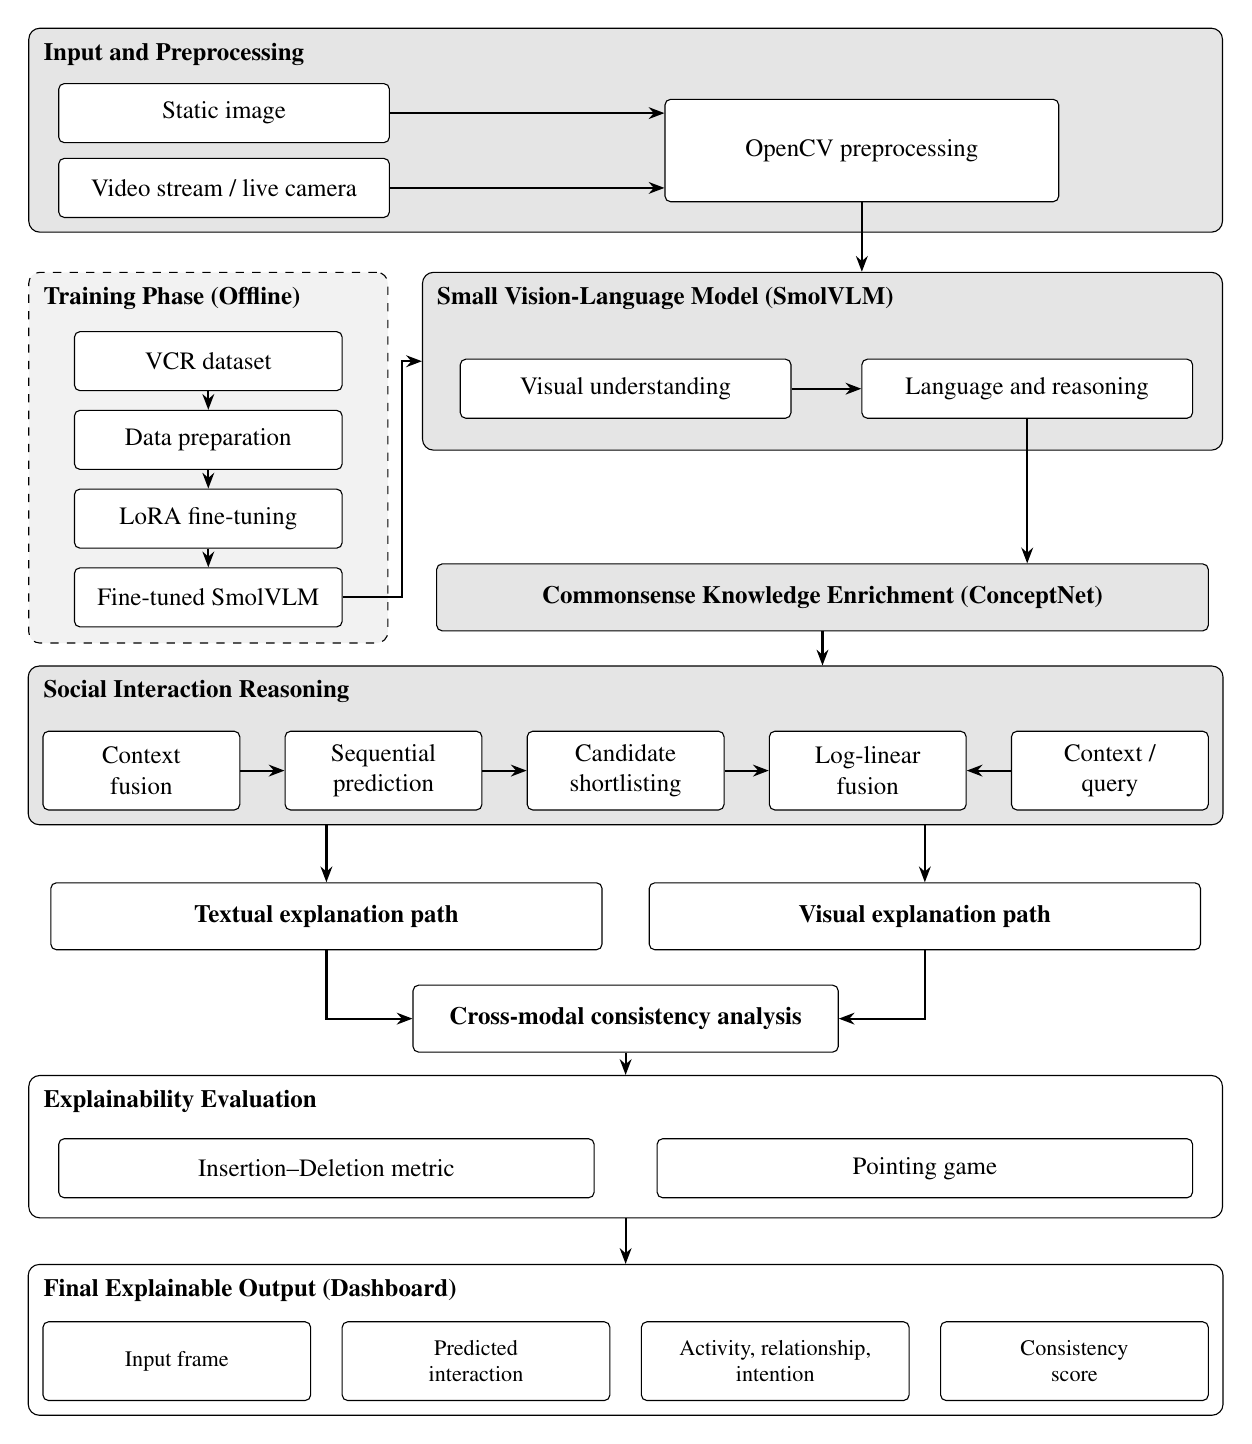
\begin{tikzpicture}[
  font=\small, >={Stealth[length=2mm]},
  box/.style={draw, rounded corners=2pt, fill=white, align=center,
              minimum height=0.75cm, inner sep=3pt},
  grp/.style={draw, rounded corners=4pt, inner sep=0.18cm},
  p1/.style={grp, fill=phaseone},
  p2/.style={grp, fill=white},
  ttl/.style={anchor=west, font=\small\bfseries, inner sep=0pt},
  arr/.style={->, thick}
]
%% ---- Input and preprocessing (Phase I)
\node[ttl] (t1) at (0.6,0.75) {Input and Preprocessing};
\node[box, minimum width=4.2cm] (in1) at (2.9,0.0) {Static image};
\node[box, minimum width=4.2cm] (in2) at (2.9,-0.95) {Video stream / live camera};
\node[box, minimum width=5cm, minimum height=1.3cm] (pre) at (11,-0.475) {OpenCV preprocessing};
\coordinate (c1a) at (0.6,0.75); \coordinate (c1b) at (15.4,-1.33);
\begin{scope}[on background layer]
  \node[p1, fit=(t1)(in1)(in2)(pre)(c1a)(c1b)] (g1) {};
\end{scope}
\draw[arr] (in1.east) -- (in1.east -| pre.west);
\draw[arr] (in2.east) -- (in2.east -| pre.west);

%% ---- Offline training phase
\node[ttl] (t2) at (0.6,-2.35) {Training Phase (Offline)};
\node[box, minimum width=3.4cm] (tr1) at (2.7,-3.15) {VCR dataset};
\node[box, minimum width=3.4cm] (tr2) at (2.7,-4.15) {Data preparation};
\node[box, minimum width=3.4cm] (tr3) at (2.7,-5.15) {LoRA fine-tuning};
\node[box, minimum width=3.4cm] (tr4) at (2.7,-6.15) {Fine-tuned SmolVLM};
\coordinate (c2a) at (0.6,-2.35); \coordinate (c2b) at (4.8,-6.55);
\begin{scope}[on background layer]
  \node[grp, dashed, fill=phaseone!50, fit=(t2)(tr1)(tr4)(c2a)(c2b)] (g2) {};
\end{scope}
\draw[arr] (tr1) -- (tr2);
\draw[arr] (tr2) -- (tr3);
\draw[arr] (tr3) -- (tr4);

%% ---- SmolVLM
\node[ttl] (t3) at (5.6,-2.35) {Small Vision-Language Model (SmolVLM)};
\node[box, minimum width=4.2cm] (v1) at (8.0,-3.5) {Visual understanding};
\node[box, minimum width=4.2cm] (v2) at (13.1,-3.5) {Language and reasoning};
\coordinate (c3a) at (5.6,-2.35); \coordinate (c3b) at (15.4,-4.1);
\begin{scope}[on background layer]
  \node[p1, fit=(t3)(v1)(v2)(c3a)(c3b)] (g3) {};
\end{scope}
\draw[arr] (pre.south) -- (pre.south |- g3.north);
\draw[arr] (v1) -- (v2);
\draw[arr] (tr4.east) -- ++(0.75,0) |- (g3.west);

%% ---- ConceptNet
\node[box, fill=phaseone, font=\small\bfseries, minimum width=9.8cm,
      minimum height=0.85cm] (cn) at (10.5,-6.15)
      {Commonsense Knowledge Enrichment (ConceptNet)};
\draw[arr] (v2.south) -- (v2.south |- cn.north);

%% ---- Social interaction reasoning
\node[ttl] (t4) at (0.6,-7.35) {Social Interaction Reasoning};
\node[box, minimum width=2.5cm, minimum height=1.0cm] (s1) at (1.85,-8.35)  {Context\\fusion};
\node[box, minimum width=2.5cm, minimum height=1.0cm] (s2) at (4.925,-8.35) {Sequential\\prediction};
\node[box, minimum width=2.5cm, minimum height=1.0cm] (s3) at (8.0,-8.35)   {Candidate\\shortlisting};
\node[box, minimum width=2.5cm, minimum height=1.0cm] (s4) at (11.075,-8.35){Log-linear\\fusion};
\node[box, minimum width=2.5cm, minimum height=1.0cm] (s5) at (14.15,-8.35) {Context /\\query};
\coordinate (c4a) at (0.6,-7.35); \coordinate (c4b) at (15.4,-8.85);
\begin{scope}[on background layer]
  \node[p1, fit=(t4)(s1)(s5)(c4a)(c4b)] (g4) {};
\end{scope}
\draw[arr] (s1) -- (s2);
\draw[arr] (s2) -- (s3);
\draw[arr] (s3) -- (s4);
\draw[arr] (s5) -- (s4);
\draw[arr] (cn.south) -- (cn.south |- g4.north);

%% ---- Phase II: explanation paths and consistency
\node[box, font=\small\bfseries, minimum width=7cm, minimum height=0.85cm] (tex) at (4.2,-10.2) {Textual explanation path};
\node[box, font=\small\bfseries, minimum width=7cm, minimum height=0.85cm] (vis) at (11.8,-10.2) {Visual explanation path};
\draw[arr] (tex.north |- g4.south) -- (tex.north);
\draw[arr] (vis.north |- g4.south) -- (vis.north);
\node[box, font=\small\bfseries, minimum width=5.4cm, minimum height=0.85cm] (cons) at (8,-11.5) {Cross-modal consistency analysis};
\draw[arr] (tex.south) |- (cons.west);
\draw[arr] (vis.south) |- (cons.east);

%% ---- Phase II: evaluation
\node[ttl] (t5) at (0.6,-12.55) {Explainability Evaluation};
\node[box, minimum width=6.8cm] (e1) at (4.2,-13.4)  {Insertion--Deletion metric};
\node[box, minimum width=6.8cm] (e2) at (11.8,-13.4) {Pointing game};
\coordinate (c5a) at (0.6,-12.55); \coordinate (c5b) at (15.4,-13.85);
\begin{scope}[on background layer]
  \node[p2, fit=(t5)(e1)(e2)(c5a)(c5b)] (g5) {};
\end{scope}
\draw[arr] (cons.south) -- (cons.south |- g5.north);

%% ---- Phase II: dashboard
\node[ttl] (t6) at (0.6,-14.95) {Final Explainable Output (Dashboard)};
\node[box, font=\footnotesize, minimum width=3.4cm, minimum height=1.0cm] (d1) at (2.3,-15.85)  {Input frame};
\node[box, font=\footnotesize, minimum width=3.4cm, minimum height=1.0cm] (d2) at (6.1,-15.85)  {Predicted\\interaction};
\node[box, font=\footnotesize, minimum width=3.4cm, minimum height=1.0cm] (d3) at (9.9,-15.85)  {Activity, relationship,\\intention};
\node[box, font=\footnotesize, minimum width=3.4cm, minimum height=1.0cm] (d4) at (13.7,-15.85) {Consistency\\score};
\coordinate (c6a) at (0.6,-14.95); \coordinate (c6b) at (15.4,-16.35);
\begin{scope}[on background layer]
  \node[p2, fit=(t6)(d1)(d4)(c6a)(c6b)] (g6) {};
\end{scope}
\draw[arr] (cons.south |- g5.south) -- (cons.south |- g6.north);
\end{tikzpicture}%
}
\caption{Architecture Design of Proposed System (shaded: Phase I; unshaded: Phase II)}
\label{fig:architecture}
\end{figure}

% -----------------------------------------
\section{PHASE I ARCHITECTURE}

The part of the architecture implemented in Phase I is shown in Figure~\ref{fig:phase1}. The modules are connected through structured Python data objects rather than by passing unstructured text between stages. The main implementation files are listed in Table~\ref{tab:codemap}.

\begin{figure}[H]
\centering
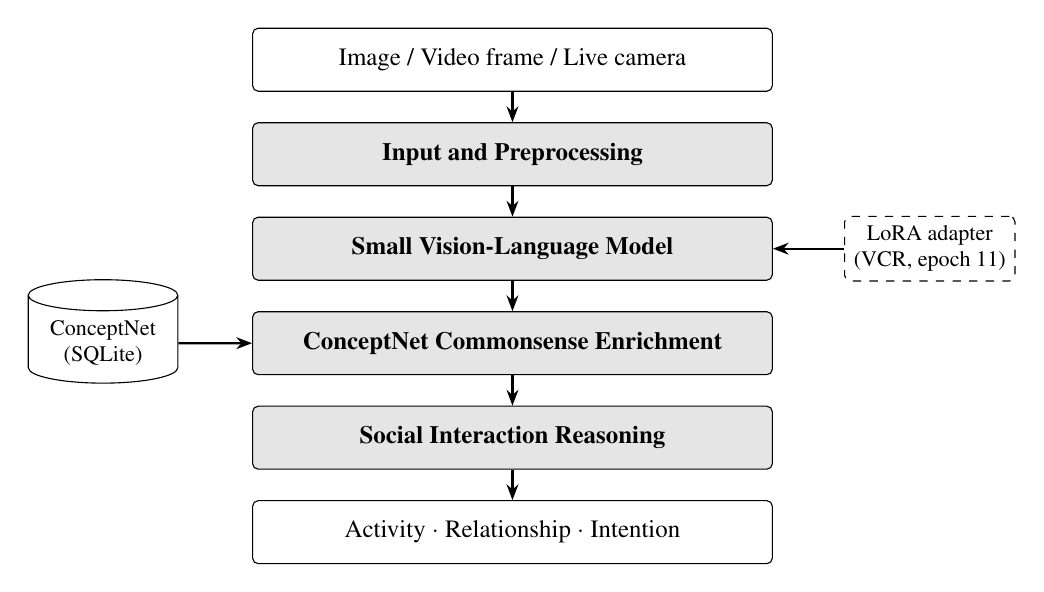
\begin{tikzpicture}[
  font=\small, >={Stealth[length=2mm]},
  box/.style={draw, rounded corners=2pt, align=center, minimum height=0.8cm,
              minimum width=6.6cm, inner sep=3pt},
  mod/.style={box, fill=phaseone, font=\small\bfseries},
  arr/.style={->, thick}
]
\node[box] (a0) at (0,0) {Image / Video frame / Live camera};
\node[mod] (a1) at (0,-1.2) {Input and Preprocessing};
\node[mod] (a2) at (0,-2.4) {Small Vision-Language Model};
\node[mod] (a3) at (0,-3.6) {ConceptNet Commonsense Enrichment};
\node[mod] (a4) at (0,-4.8) {Social Interaction Reasoning};
\node[box] (a5) at (0,-6.0) {Activity $\cdot$ Relationship $\cdot$ Intention};
\draw[arr] (a0) -- (a1);
\draw[arr] (a1) -- (a2);
\draw[arr] (a2) -- (a3);
\draw[arr] (a3) -- (a4);
\draw[arr] (a4) -- (a5);
\node[draw, cylinder, shape border rotate=90, aspect=0.25, minimum height=1.3cm,
      minimum width=1.9cm, align=center, font=\footnotesize] (db) at (-5.2,-3.6)
      {ConceptNet\\(SQLite)};
\draw[arr] (db.east) -- (a3.west);
\node[draw, dashed, rounded corners=2pt, align=center, font=\footnotesize,
      minimum height=0.8cm] (lora) at (5.3,-2.4) {LoRA adapter\\(VCR, epoch 11)};
\draw[arr] (lora.west) -- (a2.east);
\end{tikzpicture}
\caption{Phase I Architecture}
\label{fig:phase1}
\end{figure}

\begin{table}[h!]
\centering
\caption{Phase I Module-to-Code Mapping}
\label{tab:codemap}
\small
\renewcommand{\arraystretch}{1.3}
\begin{tabularx}{\textwidth}{|p{5.6cm}|L|}
\hline
\textbf{Module} & \textbf{Implementation}\\ \hline
Input and Preprocessing & \path{svcr/preprocessing.py}, \code{Preprocessor}, \code{FrameStream}\\ \hline
Small Vision-Language Model & \path{svcr/vlm.py}, \code{SmolVLMEngine}\\ \hline
ConceptNet Commonsense Enrichment & \path{svcr/conceptnet/client.py}, \path{enrichment.py}, \path{relations.py}\\ \hline
Social Interaction Reasoning & \path{svcr/reasoning.py}, \code{SocialInteractionReasoner}\\ \hline
Fine-Tuning (offline) & \path{finetune/train_vcr_lora.py}, \path{configs/finetuned.yaml}\\ \hline
Pipeline Integration & \path{svcr/pipeline.py}, \code{Phase1Pipeline}\\ \hline
Data Structures & \path{svcr/schemas.py}\\ \hline
Configuration & \path{configs/default.yaml}, \path{configs/taxonomy.yaml}\\ \hline
\end{tabularx}
\end{table}

% -----------------------------------------
\section{DATA FLOW}

For a single image, data flows through the pipeline as follows. The image is acquired and its quality is assessed; the necessary preprocessing is applied, and the frame is converted into the RGB representation expected by the model together with a normalised tensor. SmolVLM then examines the frame to identify the people, objects, actions, gestures, setting and spatial relationships, and produces a draft activity, relationship, intention and rationale, as well as an answer to the user's question when one is asked.

Salient concepts are next extracted from these outputs and looked up in ConceptNet. The useful commonsense relations are retained and used to calculate the support for each candidate label in the taxonomy. Finally, the VLM probabilities, the ConceptNet support and the draft-matching scores are fused to predict the activity, relationship and intention in sequence, and the structured result is returned with its evidence, alternatives, explanation and timings.

% -----------------------------------------
\section{MODULES}

The Phase I system consists of the following modules: Input and Preprocessing, the Small Vision-Language Model, Fine-Tuning on VCR (offline), ConceptNet Commonsense Enrichment, Social Interaction Reasoning, and the Phase I Integration that connects them.

\subsection{Input and Preprocessing Module}
\label{sec:preproc}

The Input and Preprocessing module provides a common input representation for all downstream components. It is implemented in \path{svcr/preprocessing.py} using OpenCV~\cite{bradski2000opencv}, NumPy and, where required, PIL.

\subsubsection{Input Sources}
The module accepts image file paths, HTTP and HTTPS image URLs, NumPy arrays and PIL images, as well as video files and live camera streams. Each is converted into a common BGR frame before further processing.

\subsubsection{Quality Assessment}
For every frame the brightness, contrast and blur are calculated; blur is estimated from the variance of the Laplacian. Frames that are dark or low in contrast are enhanced by applying CLAHE~\cite{zuiderveld1994clahe} to the luminance channel of the LAB colour space, followed by a mild gamma correction. Optional non-local-means denoising is available through the configuration.

\subsubsection{Resize and Normalisation}
The default resizing mode preserves the aspect ratio and limits the longest side to a size compatible with the model. The RGB image is retained as an 8-bit image for the SmolVLM processor, and a normalised tensor is also generated:
\begin{equation}
  x_{\text{norm}} = \frac{x/255 - \mu}{\sigma}, \qquad
  \mu = \sigma = (0.5, 0.5, 0.5)
  \label{eq:norm}
\end{equation}
The tensor has shape $1 \times 3 \times H \times W$ and is retained for the Phase II operations, Grad-CAM and Insertion--Deletion. The procedure is given in Algorithm~\ref{alg:preprocess}.

\begin{algorithm}[H]
\caption{Input Preprocessing}
\label{alg:preprocess}
\begin{algorithmic}[1]
\Require Image source $S$ (path, URL, array or PIL image); target longest side $N$; normalisation constants $\mu,\sigma$
\Ensure Preprocessed frame $F$
\State $I \gets \textsc{LoadAsBGR}(S)$;\; $(h,w) \gets$ size of $I$
\State $g \gets$ greyscale version of $I$
\State $b \gets \operatorname{mean}(g)$;\; $c \gets \operatorname{std}(g)$;\; $z \gets \operatorname{Var}(\nabla^2 g)$ \Comment{brightness, contrast, blur}
\If{$b < 60$ \textbf{or} $c < 25$}
  \State $I \gets$ CLAHE on the L channel of LAB, then gamma $0.8$
\EndIf
\If{denoising is enabled}
  \State $I \gets \textsc{NonLocalMeansDenoise}(I)$
\EndIf
\State $s \gets N / \max(h,w)$
\If{$s < 1$}
  \State $I \gets \textsc{Resize}(I, s)$ \Comment{aspect ratio preserved}
\EndIf
\State $R \gets \textsc{BGRtoRGB}(I)$
\State $T \gets (R/255 - \mu)/\sigma$, arranged as $1 \times 3 \times H \times W$
\State \Return $F = \big(R, T, (w,h), s, \{b, c, z, \text{blurry} = z < 60\}\big)$
\end{algorithmic}
\end{algorithm}

\subsubsection{Video and Live-Camera Handling}
For video and live-camera input, \code{FrameStream} samples frames at a configurable interval. Blurry frames can be skipped, and frames that show the same scene as the last analysed frame are filtered out using the Bhattacharyya distance between HSV histograms, with a periodic refresh so that a scene is not suppressed indefinitely (Algorithm~\ref{alg:framesample}). For uploaded videos, the web interface selects up to seven key moments: the clip is divided into scene segments using colour histograms, and the sharpest frame from the central part of each segment is analysed.

\begin{algorithm}[H]
\caption{Frame Sampling for Video and Live Camera}
\label{alg:framesample}
\begin{algorithmic}[1]
\Require Frame stream $\{(f_t, t)\}$; interval $\Delta$; scene-change threshold $\tau$
\Ensure Sequence of frames to analyse
\State $t_{\text{check}} \gets -\infty$;\; $t_{\text{last}} \gets -\infty$;\; $H_{\text{last}} \gets \textsc{null}$
\ForAll{frames $(f_t, t)$ in the stream}
  \If{$t - t_{\text{check}} < \Delta$ \textbf{or} $f_t$ is blurry}
    \State \textbf{continue}
  \EndIf
  \State $t_{\text{check}} \gets t$;\; $H \gets$ HSV histogram of $f_t$
  \If{$H_{\text{last}} \neq \textsc{null}$ \textbf{and} $t - t_{\text{last}} < 3\Delta$ \textbf{and} $d_{\text{Bhatt}}(H_{\text{last}}, H) < \tau$}
    \State \textbf{continue} \Comment{same scene as last analysed frame}
  \EndIf
  \State $t_{\text{last}} \gets t$;\; $H_{\text{last}} \gets H$
  \State \textbf{output} $f_t$
\EndFor
\end{algorithmic}
\end{algorithm}

\subsection{Small Vision-Language Model Module}
\label{sec:vlm}

The VLM module is implemented by \code{SmolVLMEngine} in \path{svcr/vlm.py}. The default configuration uses \code{HuggingFaceTB/SmolVLM-Instruct}, loaded through Hugging Face Transformers~\cite{wolf2020transformers}. The engine loads the model and processor once, selects CUDA, MPS or the CPU as available, and provides three operations: \code{generate()} for deterministic text generation, \code{score\_options()} for multiple-choice probability estimation, and \code{run()}, which performs the complete visual-understanding and draft-reasoning stage.

\subsubsection{Visual Understanding}
The engine first generates a detailed, people-centric description of the image. Short follow-up prompts then ask for the number of people, the important objects, the actions being performed, the facial expressions, gestures and body language, the setting, and a description or role for each person. The answers are parsed into clean concept lists and stored in a \code{VisualConcepts} object; text utilities normalise the phrases and extract spatial relationships from the description.

\subsubsection{Language and Reasoning}
The second sub-stage generates free-form draft answers for the activity, the relationship and the intention, a visual rationale that explains them, and an answer to the user's question when one is provided. Decoding is deterministic: sampling is disabled and a repetition penalty is applied, so the same input always gives the same output. Algorithm~\ref{alg:vlm} gives the procedure; \textsc{Generate} denotes greedy decoding with a repetition penalty.

\begin{algorithm}[H]
\caption{Visual Understanding and Draft Reasoning with SmolVLM}
\label{alg:vlm}
\begin{algorithmic}[1]
\Require Preprocessed frame $F$; optional question $Q$
\Ensure Visual concepts $V$; draft reasoning $D$
\State $cap \gets \textsc{Generate}(F, \text{describe-the-people prompt})$
\State $\theta \gets \textsc{ExtractTerms}(cap)$ \Comment{nouns, verbs, adjectives, people}
\ForAll{$k \in \{\text{count, objects, actions, gestures, setting, people}\}$}
  \State $a_k \gets \textsc{Generate}(F, \text{prompt}_k)$
\EndFor
\State $n \gets \textsc{ParseCount}(a_{\text{count}})$; if no number is found, $n \gets \textsc{ParseCount}(cap)$
\State $V.\mathit{objects} \gets \textsc{Split}(a_{\text{objects}}) \cup \theta.\text{nouns}$
\State $V.\mathit{actions} \gets \textsc{Split}(a_{\text{actions}}) \cup \theta.\text{verbs}$
\State $V.\mathit{gestures} \gets \textsc{Split}(a_{\text{gestures}})$;\; $V.\mathit{people} \gets \textsc{Split}(a_{\text{people}}) \cup \theta.\text{people}$
\State $V.\mathit{setting} \gets a_{\text{setting}}$;\; $V.\mathit{spatial} \gets \textsc{SpatialRelations}(cap)$
\If{$n \geq 2$}
  \State $D.\mathit{activity} \gets \textsc{Generate}(F, \text{``what interaction is happening?''})$
  \State $D.\mathit{relationship} \gets \textsc{Generate}(F, \text{``what is their relationship?''})$
\Else
  \State $D.\mathit{activity} \gets \textsc{Generate}(F, \text{``what is the person doing?''})$
  \State $D.\mathit{relationship} \gets \text{``no relationship''}$
\EndIf
\State $D.\mathit{intention} \gets \textsc{Generate}(F, \text{``why are they } D.\mathit{activity}\text{?''})$
\State $D.\mathit{rationale} \gets \textsc{Generate}(F, \text{``what visible evidence shows this?''})$
\If{$Q \neq \textsc{null}$}
  \State $q' \gets Q$ + ``answer briefly and give the visual reason''
  \State $D.\mathit{answer} \gets \textsc{Generate}(F, q')$
\EndIf
\State \Return $(V, D)$
\end{algorithmic}
\end{algorithm}

\subsubsection{Multiple-Choice Scoring}
For a multiple-choice question the engine reads the next-token logits for the option letters instead of generating text. The resulting option probabilities are averaged over several orderings of the options to reduce letter and position bias (Algorithm~\ref{alg:mcscore}), and are later used by the reasoning module.

\begin{algorithm}[H]
\caption{Debiased Multiple-Choice Scoring}
\label{alg:mcscore}
\begin{algorithmic}[1]
\Require Frame $F$; question $q$; options $o_1,\dots,o_n$; context $c$; number of orderings $k$
\Ensure Probabilities $p_1,\dots,p_n$ with $\sum_i p_i = 1$
\If{$n = 1$}
  \State \Return $(1)$
\EndIf
\State $\Pi \gets \{\text{identity order}\}$; if $k \geq 2$, add the reversed order and $k-2$ cyclic shifts
\State $p \gets (0,\dots,0)$
\ForAll{orderings $\pi \in \Pi$}
  \State $\mathit{prompt} \gets c + q +$ one line ``letter$_i$. $o_{\pi(i)}$'' for each option
  \State append ``Answer with the letter of the best option.'' to $\mathit{prompt}$
  \State $z \gets$ next-token logits of SmolVLM for $(F, \mathit{prompt})$
  \For{$i = 1$ \textbf{to} $n$}
    \State $\ell_i \gets \max_{t \in \text{tokens}(\text{letter}_i)} z_t$
  \EndFor
  \State $s \gets \operatorname{softmax}(\ell)$
  \For{$i = 1$ \textbf{to} $n$}
    \State $p_{\pi(i)} \gets p_{\pi(i)} + s_i$ \Comment{map back to the original option}
  \EndFor
\EndFor
\State \Return $p / |\Pi|$
\end{algorithmic}
\end{algorithm}

\subsection{Fine-Tuning on VCR (Offline)}
\label{sec:finetune}

Used zero-shot, SmolVLM sometimes gives reasons that the image does not support. To adapt it to commonsense reasoning about people, the model is fine-tuned on the VCR dataset~\cite{zellers2019vcr} with LoRA~\cite{hu2022lora} (Equation~\ref{eq:lora}). Low-rank adapters of rank 16 are added to the attention and feed-forward projections of the language model, while the SigLIP vision encoder and the connector stay frozen, so only a small fraction of the parameters is trained (about 18.1 million trainable parameters).

\subsubsection{Data Preparation}
The people and objects referred to in each VCR question are drawn on the image as labelled boxes (\emph{person1}, \emph{person2}, and so on), and the question text uses the same tags. Three kinds of training example are built from each question: multiple-choice question answering (\QtoA), multiple-choice selection of the rationale for the correct answer (\QAtoR), and a free-form answer followed by its visual reason. The multiple-choice prompts are word for word the prompts used by the option scoring of Algorithm~\ref{alg:mcscore}, so training directly sharpens the probabilities that the reasoning module fuses. The order of the options is shuffled so that no letter is favoured, and the loss is computed only on the answer tokens.

\subsubsection{Training and Checkpoint Selection}
The model is trained for 20 epochs. After every epoch the adapter is saved and scored on a selection set of VCR validation questions, and the epoch with the highest \QtoAR{} accuracy is kept; ties are broken by higher \QtoA{} accuracy and then by the earlier epoch. The final accuracy is measured on a separate test set of held-out validation questions, so the choice of epoch does not bias the reported result (Algorithm~\ref{alg:lora}). In the completed run, epoch 11 was selected. The selected adapter is merged into the base weights when the model is loaded through \path{configs/finetuned.yaml}, so inference with the fine-tuned model is as fast as with the base model.

\subsubsection{Implementation}
The procedure is implemented in \path{finetune/train_vcr_lora.py}. The script streams VCR images from the dataset's Parquet files, draws the labelled boxes, builds the three kinds of training example and caches the prepared data. It saves a checkpoint every 50 steps so that an interrupted run can be resumed, and records the training loss, the per-epoch selection accuracy and the final test accuracy. After the run, \path{install_adapter.py} copies the selected adapter into the project. The configuration is listed in Table~\ref{tab:ftconfig}.

\begin{table}[h!]
\centering
\caption{Fine-Tuning Configuration}
\label{tab:ftconfig}
\small
\renewcommand{\arraystretch}{1.3}
\begin{tabularx}{\textwidth}{|p{4.2cm}|L|}
\hline
\textbf{Setting} & \textbf{Value}\\ \hline
Base model & \code{HuggingFaceTB/SmolVLM-Instruct} (2.2B parameters)\\ \hline
Adapter & LoRA, rank 16, alpha 32, dropout 0.05\\ \hline
Adapted layers & Query, key, value, output, gate, up and down projections of the language model\\ \hline
Frozen components & SigLIP vision encoder and connector\\ \hline
Training data & Hugging Face VCR dataset (\QtoA, \QAtoR{} and explanation examples)\\ \hline
Image resolution & Longest edge 768 pixels\\ \hline
Batch size & 2, with gradient accumulation over 8 steps (effective batch of 16)\\ \hline
Optimiser & AdamW, learning rate $10^{-4}$, cosine schedule with 5\% warm-up\\ \hline
Training length & 20 epochs of 75 steps (1,500 optimiser steps)\\ \hline
Checkpoint selection & Best \QtoAR{} on selection questions: epoch 11\\ \hline
Test set & Held-out VCR validation questions\\ \hline
\end{tabularx}
\end{table}

\begin{algorithm}[H]
\caption{LoRA Fine-Tuning with Best-Epoch Selection}
\label{alg:lora}
\begin{algorithmic}[1]
\Require Base model $M$; training examples $X$; selection set $S_{\text{sel}}$; test set $S_{\text{test}}$; number of epochs $E = 20$
\Ensure Selected adapter $A^*$; test accuracy before and after fine-tuning
\State add LoRA adapters to the language model of $M$; freeze all other weights
\State $r_{\text{base}} \gets \textsc{Evaluate}(M \text{ without adapters}, S_{\text{test}})$
\For{$e = 1$ \textbf{to} $E$}
  \ForAll{mini-batches $B \subset X$}
    \State update the adapters to minimise the cross-entropy of the answer tokens of $B$
  \EndFor
  \State $A_e \gets$ current adapters;\; $r_e \gets \textsc{Evaluate}(M + A_e, S_{\text{sel}})$
\EndFor
\State $e^* \gets \arg\max_e \big(r_e.\text{\QtoAR},\; r_e.\text{\QtoA},\; -e\big)$ \Comment{ties: higher \QtoA, then earlier epoch}
\State $A^* \gets A_{e^*}$;\; $r_{\text{ft}} \gets \textsc{Evaluate}(M + A^*, S_{\text{test}})$
\State \Return $A^*, r_{\text{base}}, r_{\text{ft}}$
\end{algorithmic}
\end{algorithm}

\subsection{ConceptNet Commonsense Enrichment Module}
\label{sec:conceptnet}

Visual observations alone may not be enough to distinguish semantically similar interactions. The enrichment module uses ConceptNet~\cite{speer2017conceptnet} to add commonsense knowledge to the visual concepts and produces evidence that is fused into the final prediction. It is divided into a client layer, which handles backend access, caching, term normalisation and phrase back-off, and an enrichment layer, which assigns salience, filters evidence and computes label support.

\subsubsection{Key-Term Extraction}
Candidate terms are collected from the actions, gestures, roles, objects and setting identified by the VLM, from its description and draft answers, and from the user's question. Each term receives a salience weight, highest for interaction-relevant kinds such as actions (1.0) and gestures (0.9).

\subsubsection{ConceptNet Backend}
Three backends are supported: a local SQLite copy of ConceptNet, the public ConceptNet API with a persistent on-disk cache, and an offline mode in which taxonomy-based keyword matching remains available. The local backend is preferred for reproducibility whenever the database is present. An unknown phrase such as ``shaking hands'' is retried as \code{shake\_hands} and then as its head word.

\subsubsection{Relevance Filtering}
For each term the module retrieves its edges and filters them by relation type and weight. Facts that link the term to the anchor concepts of the social-interaction labels, or to other concepts observed in the same image, are ranked highest. Generic hub concepts, which are connected to almost everything, are suppressed because they carry little discriminative value.

\subsubsection{Label Support and Ambiguity Resolution}
For each activity, relationship and intention label, the module calculates how strongly the evidence supports it (Algorithm~\ref{alg:support}). A term contributes support if it is one of the label's anchor concepts, if a direct edge connects it to an anchor, if its two-hop neighbourhood overlaps that of the label, or if it matches one of the label's keywords, weighted by inverse document frequency. Negative relations such as \emph{Antonym} and \emph{DistinctFrom} reduce the support. The module therefore produces a numerical support score for every label together with readable evidence paths, and combines the support with the match to the VLM draft to produce a preliminary disambiguated label for each task (Algorithm~\ref{alg:enrich}). The taxonomy, including each label's anchors and keywords, is kept in \path{configs/taxonomy.yaml} so that it can be changed without modifying the code.

\begin{algorithm}[H]
\caption{ConceptNet Commonsense Enrichment}
\label{alg:enrich}
\begin{algorithmic}[1]
\Require Visual concepts $V$; draft $D$; optional question $Q$; taxonomy $\mathcal{T}$
\Ensure Facts $\mathcal{F}$; support $S$; draft match $M$; evidence; disambiguated labels $\hat{L}$
\State $E \gets$ terms from $V$, $D$ and $Q$, each with a salience (action 1.0, gesture 0.9, role 0.9, object 0.7, setting 0.6, caption 0.5); keep the top 20
\ForAll{terms $e \in E$}
  \State $(c_e, \mathit{edges}_e) \gets \textsc{Resolve}(e)$ \Comment{phrase $\rightarrow$ lemma $\rightarrow$ head word}
  \If{$c_e$ is shorter than $e$}
    \State $\mathrm{salience}(e) \gets 0.5 \cdot \mathrm{salience}(e)$ \Comment{backed-off sense is less reliable}
  \EndIf
  \State $P_e[v] \gets w_{\text{rel}} \cdot (1 - e^{-\text{weight}})$ for each neighbour $v$ that is not a generic hub
  \State $N_e \gets$ neighbours linked by \emph{Antonym}, \emph{DistinctFrom} or \emph{Not*} relations
\EndFor
\State $\mathcal{F} \gets$ top 6 facts per term, ranked by relevance ($\times 2$ if the neighbour is a label anchor, $\times 1.5$ if it is another observed concept); keep the top 40
\ForAll{tasks $\tau \in \{\text{activity, relationship, intention}\}$}
  \ForAll{labels $L \in \mathcal{T}[\tau]$}
    \State $S_\tau(L) \gets \dfrac{\sum_e w_{e,\tau}\, \textsc{Score}(e, L)}{\sum_e w_{e,\tau}}$ \Comment{Algorithm~\ref{alg:support}}
    \State $M_\tau(L) \gets \max\big(\mathrm{lex}(D_\tau, L),\; 0.8 \max_{e \in \text{draft}} \textsc{Score}(e, L)\big)$
  \EndFor
  \State $S_\tau \gets S_\tau / \max\big(\max_L S_\tau(L),\, 0.3\big)$
  \State $\hat{L}_\tau \gets \arg\max_L \big(S_\tau(L) + M_\tau(L)\big)$
\EndFor
\State \Return $\mathcal{F}, S, M$, evidence paths, $\hat{L}$
\end{algorithmic}
\end{algorithm}

Here $w_{e,\tau}$ is the salience of term $e$ multiplied by the weight of its kind for task $\tau$; for example, roles count most for the relationship task and actions most for the activity task.

\begin{algorithm}[H]
\caption{Support of One Evidence Term for One Label}
\label{alg:support}
\begin{algorithmic}[1]
\Require Term $e$ with concept $c_e$, neighbour profile $P_e$ and negative neighbours $N_e$; label $L$ with anchors $A_L$, lexicon $X_L$ and neighbour profile $P_L$
\Ensure Support score $s$
\If{$c_e \in A_L$}
  \State \Return $1.0$ \Comment{exact anchor}
\EndIf
\State $s \gets 0$
\ForAll{anchors $a \in A_L$}
  \If{$a \in P_e$}
    \State $s \gets \max(s,\, 0.9\, P_e[a])$ \Comment{direct edge}
  \EndIf
\EndFor
\State $s \gets \max\big(s,\; 0.6 \cdot \min(1,\, 2.5 \cos(P_e, P_L))\big)$ \Comment{two-hop overlap}
\State $H \gets \mathrm{words}(e) \cap X_L$
\If{$H \neq \emptyset$}
  \State $s \gets \max\big(s,\; 0.6 / \min_{w \in H} \mathrm{df}(w)\big)$ \Comment{keyword, IDF-weighted}
\EndIf
\If{$N_e \cap A_L \neq \emptyset$}
  \State $s \gets s - 0.5$ \Comment{contradicting relation}
\EndIf
\State \Return $s$
\end{algorithmic}
\end{algorithm}

\subsection{Social Interaction Reasoning Module}
\label{sec:reasoning}

The Social Interaction Reasoning module, \code{SocialInteractionReasoner}, is the fusion point of Phase I. It combines the visual concepts, the commonsense evidence, the VLM draft and the optional user question to predict the social interaction.

\subsubsection{Context Fusion}
The module builds a structured context from the scene description, the number of people and their descriptions, the actions, gestures, objects and setting identified by the VLM, a selection of the most relevant ConceptNet facts, and the user's question. This context accompanies the image in every prompt that the module sends to the VLM.

\subsubsection{Sequential Prediction}
The three tasks are inferred in the order activity, relationship, intention. The predicted activity is added to the context for relationship inference, and both the activity and the relationship are added to the context for intention inference, so that each later prediction is consistent with the earlier ones.

\subsubsection{Candidate Shortlisting}
ConceptNet support, VLM draft matching and lexical evidence are combined into a prior over the taxonomy labels. When the prior is informative, only the highest-ranked candidates are shortlisted; otherwise the complete label set is passed to the VLM.

\subsubsection{Log-Linear Fusion}
Let $p_{\text{VLM}}(L)$ be the VLM probability for label $L$, $p_{\text{CN}}(L)$ the normalised ConceptNet support, and $m_{\text{draft}}(L)$ the match between the VLM draft and the label. The module computes
\begin{equation}
  \log P(L) \;\propto\; w_{\text{VLM}} \log p_{\text{VLM}}(L)
  + w_{\text{CN}} \log p_{\text{CN}}(L)
  + w_{\text{draft}}\, m_{\text{draft}}(L)
  \label{eq:fusion}
\end{equation}
with default weights $w_{\text{VLM}} = 1.0$, $w_{\text{CN}} = 0.5$ and $w_{\text{draft}} = 1.0$. The resulting distribution gives the highest-scoring label with its confidence, the ranked alternatives with their component probabilities, and the evidence behind the prediction. A prediction is marked ambiguous when the probability margin between the top two labels is below 0.15. Algorithm~\ref{alg:infertask} infers one task in this way.

\begin{algorithm}[H]
\caption{Inference of One Task with Log-Linear Fusion}
\label{alg:infertask}
\begin{algorithmic}[1]
\Require Task $\tau$; frame $F$; context $c$; visual concepts $V$; support $S_\tau$; draft match $M_\tau$; disambiguated label $\hat{L}_\tau$
\Ensure Prediction for $\tau$: label, confidence, ambiguity flag, alternatives, evidence
\State $\mathcal{L} \gets$ labels of $\tau$ (excluding \code{none\_single} for relationship)
\ForAll{$L \in \mathcal{L}$}
  \State $\mathit{prior}(L) \gets S_\tau(L) + 1.5\, M_\tau(L) + 0.3\, \mathrm{lex}(\text{scene text}, L)$
\EndFor
\If{fewer than 3 labels have $\mathit{prior} > 0.05$}
  \State $C \gets \mathcal{L}$ \Comment{no reliable prior: VLM sees all labels}
\Else
  \State $C \gets$ the 8 labels with the highest prior, always including $\hat{L}_\tau$
\EndIf
\State $p_{\text{VLM}} \gets \textsc{ScoreOptions}(F, \text{question}_\tau, \text{descriptions of } C, c)$ \Comment{Algorithm~\ref{alg:mcscore}}
\If{$\max_{L \in C} S_\tau(L) < 10^{-3}$}
  \State $p_{\text{CN}} \gets$ uniform over $C$
\Else
  \State $p_{\text{CN}} \gets \operatorname{softmax}(S_\tau / T)$, $T = 0.2$
\EndIf
\ForAll{$L \in C$}
  \State $z(L) \gets w_{\text{VLM}} \log p_{\text{VLM}}(L) + w_{\text{CN}} \log p_{\text{CN}}(L) + w_{\text{draft}}\, M_\tau(L)$
\EndFor
\State $P \gets \operatorname{softmax}(z)$; sort $C$ by $P$ in descending order
\State $L^* \gets C_1$;\; $\mathit{ambiguous} \gets \big(P(C_1) - P(C_2) < 0.15\big)$
\State \Return $\big(L^*, P(L^*), \mathit{ambiguous}, C \text{ with } P, p_{\text{VLM}}, p_{\text{CN}}, M_\tau, \text{evidence for } L^*\big)$
\end{algorithmic}
\end{algorithm}

\subsubsection{Special Cases and Explanation}
Scenes with zero or one detected person are handled explicitly. When only one person is present, the relationship is set to \code{none\_single}; when no people are detected, the system returns a no-interaction prediction instead of inferring a social relationship. Once the three tasks are inferred, an explanation is generated by a prompt that asks the VLM to relate the prediction to the visible people, gestures, facial expressions, objects and setting. Algorithm~\ref{alg:reason} applies these steps to the three tasks in sequence.

\begin{algorithm}[H]
\caption{Social Interaction Reasoning}
\label{alg:reason}
\begin{algorithmic}[1]
\Require Frame $F$; visual concepts $V$; draft $D$; commonsense result $R$; optional question $Q$ and options $O$
\Ensure Social prediction: activity, relationship, intention, explanation, answer
\State $c \gets \textsc{Fuse}(V, R, Q)$ \Comment{caption, concepts, top ConceptNet facts, question}
\If{$V.\mathit{people} = 0$}
  \State \Return no-interaction prediction
\EndIf
\State $A \gets \textsc{InferTask}(\text{activity}, F, c)$ \Comment{Algorithm~\ref{alg:infertask}}
\If{$V.\mathit{people} = 1$}
  \State $\mathit{Rel} \gets$ \code{none\_single} with confidence 1
\Else
  \State $\mathit{Rel} \gets \textsc{InferTask}(\text{relationship}, F, c + \text{``The people are } A\text{.''})$
\EndIf
\State $c' \gets c$ + ``The people are $A$. They are most likely $\mathit{Rel}$.''
\State $I \gets \textsc{InferTask}(\text{intention}, F, c')$
\State $\mathit{pr} \gets$ statement of $(A, \mathit{Rel}, I)$ + top ConceptNet facts + ``explain which visible evidence supports this''
\State $\mathit{Ex} \gets \textsc{Generate}(F, \mathit{pr})$
\If{$Q \neq \textsc{null}$ \textbf{and} $O \neq \textsc{null}$}
  \State $p \gets \textsc{ScoreOptions}(F, Q, O, c)$;\; $\mathit{ans} \gets O_{\arg\max p}$
\ElsIf{$Q \neq \textsc{null}$}
  \State $\mathit{ans} \gets D.\mathit{answer}$
\EndIf
\State \Return $(A, \mathit{Rel}, I, \mathit{Ex}, \mathit{ans})$ with the supporting evidence
\end{algorithmic}
\end{algorithm}

\subsection{Phase I Integration}

The four modules are integrated through the \code{Phase1Pipeline} class, which runs them in sequence (Algorithm~\ref{alg:pipeline}). The modules exchange structured dataclasses rather than free text: \code{PreprocessedFrame} carries the output of preprocessing, \code{VisualConcepts} and \code{DraftReasoning} carry the output of the VLM, \code{CommonsenseResult} carries the ConceptNet evidence, and \code{SocialPrediction} carries the final prediction. Together these form a \code{Phase1Result}, which can be serialised to JSON with all of its evidence and module timings.

\begin{algorithm}[H]
\caption{Phase I Pipeline}
\label{alg:pipeline}
\begin{algorithmic}[1]
\Require Input source $S$, optional question $Q$, optional answer options $O$
\Ensure Phase I result: frame, visual concepts, draft, commonsense evidence, prediction, timings
\State $F \gets \textsc{Preprocess}(S)$ \Comment{Algorithm~\ref{alg:preprocess}}
\State $(V, D) \gets \textsc{SmolVLM}(F, Q)$ \Comment{Algorithm~\ref{alg:vlm}}
\State $R \gets \textsc{EnrichWithConceptNet}(V, D, Q)$ \Comment{Algorithm~\ref{alg:enrich}}
\State $P \gets \textsc{ReasonSocialInteraction}(F, V, D, R, Q, O)$ \Comment{Algorithm~\ref{alg:reason}}
\State \Return $(F, V, D, R, P)$ with the time taken by each stage
\end{algorithmic}
\end{algorithm}

% -----------------------------------------
\section{BACKEND AND USER INTERFACE}

A FastAPI backend loads the Phase I pipeline once and keeps the model resident in memory. Each analysis runs as a background job, and the React frontend polls the job to show which module is currently running. The endpoints are listed in Appendix~\ref{app:api}.

The interface accepts an uploaded image, a photo captured from the live camera or an uploaded video, which is analysed at its key moments, together with an optional question. Results are presented as prediction cards for the activity, relationship and intention, each with its confidence value and alternatives, followed by the generated explanation, the supporting ConceptNet evidence, the visual concepts identified by the VLM and the processing time. The full result can be downloaded as a JSON report, and a history strip gives access to earlier analyses from the same session. This interface is an operational demonstration of Phase I and is distinct from the Phase II explainability dashboard.

% -----------------------------------------
\section{PLANNED PHASE II EXTENSION}
\label{sec:phase2plan}

The Phase I data flow already carries what Phase II needs: the normalised tensor of Equation~\ref{eq:norm} for visual attribution, access to the model through \code{SmolVLMEngine}, the structured prediction targets, the textual rationale and the ConceptNet evidence. Phase II will add:

\begin{itemize}
\item \textbf{Visual explanation path:} Grad-CAM~\cite{selvaraju2017gradcam} maps for each predicted label, and extraction of the concepts present in the most activated regions, giving a visual concept set $\mathcal{V}$.
\item \textbf{Textual explanation path:} extraction of the concepts mentioned in the generated explanation, giving a textual concept set $\mathcal{T}$.
\item \textbf{Cross-modal consistency:} the Jaccard overlap of the two sets,
  \begin{equation}
    \mathrm{CMC} = \frac{|\mathcal{T} \cap \mathcal{V}|}{|\mathcal{T} \cup \mathcal{V}|}
    \label{eq:cmc}
  \end{equation}
\item \textbf{Faithfulness evaluation:} the Insertion--Deletion metric~\cite{petsiuk2018rise} and the Pointing Game~\cite{zhang2018excitation}.
\item \textbf{Explainability dashboard:} the input frame, the predicted interaction, the three labels and the consistency score in a single view.
\end{itemize}
 % PROPOSED METHODOLOGY
% Chapter 4

\chapter{EXPERIMENTAL RESULTS AND PERFORMANCE ANALYSIS}
\label{ch:results}

This chapter describes the data and the computing environment used, the experiments conducted in Phase I, and an analysis of their results.

\section{DATASET DESCRIPTION}

\begin{table}[h!]
\centering
\caption{Dataset Description}
\label{tab:dataset}
\small
\renewcommand{\arraystretch}{1.3}
\begin{tabularx}{\textwidth}{|p{3.6cm}|L|}
\hline
\textbf{Attribute} & \textbf{Description} \\ \hline
Dataset & Visual Commonsense Reasoning (VCR)~\cite{zellers2019vcr}, Hugging Face release (Parquet files) \\ \hline
Source images & About 110,000 movie scenes from LSMDC~\cite{rohrbach2017lsmdc} and MovieClips \\ \hline
Questions & About 290,000 multiple-choice questions \\ \hline
Options & 4 candidate answers; 4 candidate rationales for the correct answer \\ \hline
Tasks & \QtoA, \QAtoR{} and the joint metric \QtoAR \\ \hline
Training set & VCR training split, 3 examples per question \\ \hline
Selection set & VCR validation questions, used only to choose the epoch \\ \hline
Test set & Separate held-out VCR validation questions \\ \hline
Knowledge source & ConceptNet 5.5~\cite{speer2017conceptnet}, local SQLite database \\ \hline
\end{tabularx}
\end{table}

\subsection{Visual Commonsense Reasoning (VCR) Dataset}
The VCR dataset~\cite{zellers2019vcr} contains about 290,000 multiple-choice questions over about 110,000 images taken from movie scenes, drawn from the LSMDC~\cite{rohrbach2017lsmdc} and MovieClips collections, as summarised in Table~\ref{tab:dataset}. Each question comes with four candidate answers and, for the correct answer, four candidate rationales. Objects and people in each image are detected and referred to in the text by tags, for example ``Why is [person1] pointing at [person2]?''. The questions cover explanations, activities, mental states, roles, temporal inferences and hypothetical situations, which makes them a close match to the activity, relationship and intention targets of this project. The wrong options are produced by Adversarial Matching, so they are relevant to the scene and cannot be rejected on surface cues alone.

\subsection{Data Splits Used}
Since the labels of the official VCR test split are not public, all evaluation questions are drawn from the official validation split. Three disjoint sets are used. The \textbf{training set} contains questions from the VCR training split, each expanded into a \QtoA, a \QAtoR{} and a free-form explanation example. The \textbf{selection set} of validation questions is used only to choose the epoch. The \textbf{test set} of further validation questions is used neither for training nor for choosing the epoch.

\subsection{ConceptNet Knowledge Base}
ConceptNet 5.5~\cite{speer2017conceptnet} is used as the commonsense knowledge source. A local SQLite database built from the ConceptNet assertions allows offline and reproducible lookups, with the public ConceptNet API and an on-disk cache as a fallback.

\subsection{Social Interaction Taxonomy}
The label space for the three prediction tasks is defined in \path{configs/taxonomy.yaml}. Each label has a description, a set of ConceptNet anchor concepts and a keyword lexicon. Examples of labels are \emph{Performing}, \emph{Watching together} and \emph{Photographing} for the activity; \emph{Performer or speaker and audience}, \emph{Teammates or members of the same group}, \emph{Doctor (or nurse) and patient} and \code{none\_single} for the relationship; and \emph{To entertain or perform for others}, \emph{To socialise, relax and spend time together} and \emph{To comfort, console or emotionally support someone} for the intention.
\subsection{Test Fixtures and Demonstration Data}
The automated tests use synthetic images, a deterministic stand-in for the VLM and a small ConceptNet graph, so they run without downloading the model. The qualitative demonstration uses real photographs, including the concert photograph of Section~\ref{sec:demo}.

\section{ECOSYSTEM}
\subsection{Hardware Configuration}
Fine-tuning was carried out on a GPU in the department laboratory, and the demonstration and interactive experiments were run on a local machine. The hardware configuration used is:
\begin{itemize}
    \item \textbf{Fine-tuning:} GPU workstation in the department laboratory (CUDA).
    \item \textbf{Inference and demonstration:} Apple Silicon MacBook, using the Metal Performance Shaders (MPS) backend of PyTorch.
    \item \textbf{Knowledge base storage:} local SQLite copy of ConceptNet on the inference machine, so no network access is needed at run time.
\end{itemize}

\subsection{Software Environment}
The system is organised as a Python package with separate modules for preprocessing, VLM inference, commonsense enrichment, reasoning, configuration, data structures and visualisation. The main software components used are:
\begin{itemize}
    \item \textbf{Programming Language:} Python 3.12
    \item \textbf{Image/Video Processing:} OpenCV~\cite{bradski2000opencv}, NumPy, PIL
    \item \textbf{Vision-Language Model:} SmolVLM with Hugging Face Transformers~\cite{wolf2020transformers}
    \item \textbf{Deep Learning Framework:} PyTorch~\cite{paszke2019pytorch}
    \item \textbf{Fine-Tuning:} PEFT (LoRA)
    \item \textbf{Natural-Language Processing:} spaCy and project text utilities
    \item \textbf{Commonsense Knowledge:} ConceptNet with SQLite database and cache
    \item \textbf{Backend:} FastAPI, Uvicorn
    \item \textbf{Frontend:} React, Vite, JavaScript
    \item \textbf{Testing:} pytest
    \item \textbf{Configuration:} YAML
\end{itemize}

\section{EXPERIMENTS CONDUCTED}

\subsection{Functional Validation Experiment}
The automated test suite was run with pytest to check each module and the complete pipeline. The preprocessing tests check image loading, resizing, normalisation, low-light enhancement, blur detection and frame sampling. The ConceptNet tests check term resolution, enrichment, label support and access to the local SQLite database, and further tests cover text normalisation and taxonomy loading. The end-to-end tests run the complete pipeline and check that commonsense evidence resolves the prediction when the VLM is uncertain, that scenes with one person or with no people are handled correctly, and that multiple-choice questions are answered. The video tests check key-moment selection and summarisation.

\subsection{LoRA Fine-Tuning Experiment}
SmolVLM was fine-tuned for 20 epochs with the configuration of Table~\ref{tab:ftconfig}, and the adapter was evaluated on the selection set after every epoch to choose the checkpoint.

\subsection{Quantitative Test Evaluation}
The base model and the selected fine-tuned model were evaluated on the same held-out test questions on \QtoA, \QAtoR{} and \QtoAR.

\subsection{Qualitative Comparison of Explanations}
The free-form answers and reasons of the base and fine-tuned models were compared for test questions against the reference answers.

\subsection{End-to-End Demonstration}
The integrated pipeline was run through the web interface on real photographs to inspect the predictions, the evidence and the processing time.

\section{PERFORMANCE ANALYSIS}

\subsection{Functional Validation Results}
All 23 automated tests passed, as summarised in Table~\ref{tab:tests}. These tests confirm that the module interfaces work together under controlled conditions: an input flows through preprocessing, VLM stand-in inference, ConceptNet enrichment and social reasoning to a structured prediction. Because the VLM is replaced by a deterministic stand-in, they validate the software, not the accuracy of the model; accuracy is analysed in the following sections.

\begin{table}[h!]
\centering
\caption{Automated Validation Results}
\label{tab:tests}
\small
\begin{tabular}{|l|c|c|}
\hline
\textbf{Test Category} & \textbf{Tests} & \textbf{Result}\\ \hline
Preprocessing & 7 & Passed\\ \hline
ConceptNet & 3 & Passed\\ \hline
Text and taxonomy & 5 & Passed\\ \hline
End-to-end Phase I pipeline & 5 & Passed\\ \hline
Video key-moment selection & 3 & Passed\\ \hline
\textbf{Total} & \textbf{23} & \textbf{23 Passed}\\ \hline
\end{tabular}
\end{table}

\subsection{Training Convergence}
The training loss is shown per optimiser step in Figure~\ref{fig:lossstep}, together with its moving average over 20 steps. Averaged per epoch, it falls from 2.03 in the first epoch to 0.08 in epoch 7 and 0.013 in epoch 11, and it is 0.001 or less from epoch 15 onwards. The loss therefore converges well before the end of the run.

\begin{figure}[H]
\centering
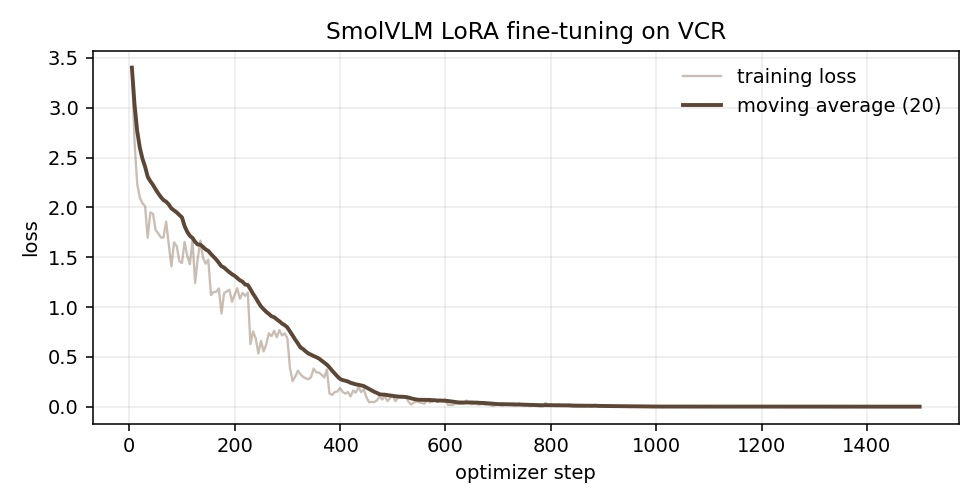
\includegraphics[width=\textwidth]{images/training_loss.png}
\caption{Training Loss of LoRA Fine-Tuning on VCR over 1,500 Optimiser Steps}
\label{fig:lossstep}
\end{figure}

\subsection{Epoch Selection}
The selection-set accuracy after every epoch is shown in Figure~\ref{fig:epochacc} and Table~\ref{tab:epochs}. Accuracy rises quickly over the first three epochs, with \QtoAR{} increasing from 33\% to 46\%, and then fluctuates between 43\% and 48\% while the training loss keeps falling. From epoch 12 onwards the accuracy is identical in every epoch, because the training loss is close to zero and the adapters no longer change.

Epochs 9 and 11 share the highest \QtoAR{} accuracy of 48\%. Epoch 11 is selected because its \QtoA{} accuracy is higher (63\% against 62\%), and its \QAtoR{} accuracy of 65\% is the second highest of the run. The final model therefore uses the epoch-11 adapter rather than the adapter from the last epoch.

\begin{figure}[H]
\centering
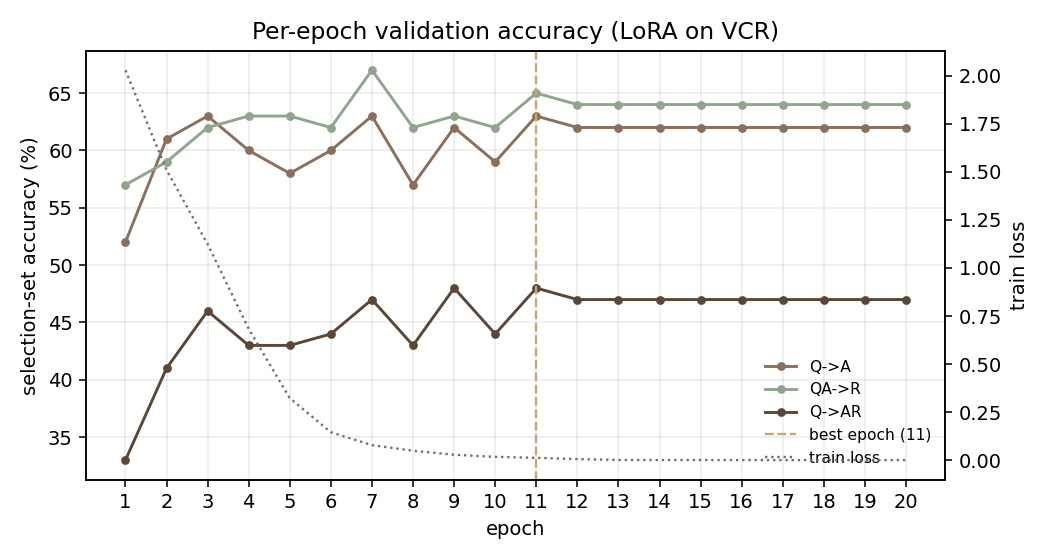
\includegraphics[width=\textwidth]{images/epoch_accuracy.jpg}
\caption{Selection-Set Accuracy and Training Loss after Each Epoch (Dashed Line: Selected Epoch 11)}
\label{fig:epochacc}
\end{figure}

\begin{table}[h!]
\centering
\caption{Per-Epoch Accuracy on the Selection Set}
\label{tab:epochs}
\small
\begin{tabular}{|c|c|c|c|c|}
\hline
\textbf{Epoch} & \textbf{Train Loss} & \textbf{\QtoA{} (\%)} & \textbf{\QAtoR{} (\%)} & \textbf{\QtoAR{} (\%)}\\ \hline
1 & 2.029 & 52 & 57 & 33\\ \hline
2 & 1.510 & 61 & 59 & 41\\ \hline
3 & 1.124 & 63 & 62 & 46\\ \hline
4 & 0.684 & 60 & 63 & 43\\ \hline
5 & 0.323 & 58 & 63 & 43\\ \hline
6 & 0.146 & 60 & 62 & 44\\ \hline
7 & 0.079 & 63 & 67 & 47\\ \hline
8 & 0.050 & 57 & 62 & 43\\ \hline
9 & 0.029 & 62 & 63 & 48\\ \hline
10 & 0.018 & 59 & 62 & 44\\ \hline
\textbf{11} & \textbf{0.013} & \textbf{63} & \textbf{65} & \textbf{48}\\ \hline
12--20 & 0.006 -- 0.001 & 62 & 64 & 47\\ \hline
\end{tabular}
\end{table}

The separation between the two curves -- training loss approaching zero while the selection accuracy stops improving after epoch 3 -- shows that the later epochs mostly fit the training examples more closely without generalising better. Selecting the epoch on held-out data, rather than using the last checkpoint, guards against this.

\subsection{Test Accuracy}
The base model and the fine-tuned model (epoch 11) were evaluated on the same held-out validation questions. Table~\ref{tab:testacc} and Figure~\ref{fig:testbar} give the results. Fine-tuning improves all three tasks by 14 to 17 percentage points, and the \QtoAR{} accuracy more than doubles, from 15.3\% to 32.7\%.

\begin{table}[h!]
\centering
\caption{Accuracy on Held-Out VCR Validation Questions}
\label{tab:testacc}
\small
\begin{tabular}{|l|c|c|c|}
\hline
\textbf{Model} & \textbf{\QtoA{} (\%)} & \textbf{\QAtoR{} (\%)} & \textbf{\QtoAR{} (\%)}\\ \hline
Chance level & 25.0 & 25.0 & 6.3\\ \hline
SmolVLM-Instruct (base) & 44.7 & 41.3 & 15.3\\ \hline
SmolVLM + LoRA (epoch 11) & \textbf{58.7} & \textbf{57.7} & \textbf{32.7}\\ \hline
Improvement (percentage points) & +14.0 & +16.3 & +17.3\\ \hline
\end{tabular}
\end{table}

\begin{figure}[H]
\centering
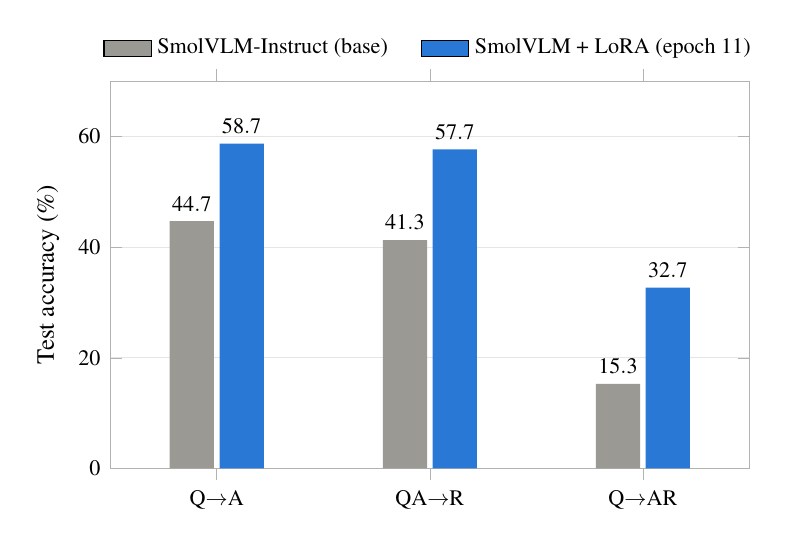
\begin{tikzpicture}
\begin{axis}[
  ybar, bar width=16pt, area legend,
  width=0.8\linewidth, height=6.5cm,
  symbolic x coords={qa,qar,qtoar},
  xtick=data, xticklabels={\QtoA, \QAtoR, \QtoAR},
  enlarge x limits=0.25,
  ymin=0, ymax=70, ylabel={Test accuracy (\%)},
  ymajorgrids, grid style={gray!20},
  axis line style={gray!60}, tick style={gray!60},
  every axis label/.style={font=\small}, ticklabel style={font=\footnotesize},
  nodes near coords, nodes near coords style={font=\footnotesize, color=black},
  every node near coord/.append style={/pgf/number format/fixed, /pgf/number format/precision=1},
  legend style={at={(0.5,1.03)}, anchor=south, legend columns=2, draw=none,
                font=\footnotesize, /tikz/every even column/.append style={column sep=10pt}},
]
\addplot[fill=neutralbar, draw=none] coordinates {(qa,44.7) (qar,41.3) (qtoar,15.3)};
\addlegendentry{SmolVLM-Instruct (base)}
\addplot[fill=seriesA, draw=none] coordinates {(qa,58.7) (qar,57.7) (qtoar,32.7)};
\addlegendentry{SmolVLM + LoRA (epoch 11)}
\end{axis}
\end{tikzpicture}
\caption{Test Accuracy of the Base and Fine-Tuned Models}
\label{fig:testbar}
\end{figure}

\subsubsection{Selection versus Test Accuracy}
The test accuracy is lower than the selection-set accuracy of epoch 11 (63\%, 65\% and 48\%). This is expected: the epoch was chosen because it scored well on the selection set, so its selection accuracy is optimistically biased. This is why the result is reported on a separate test set.

\subsubsection{Answer and Rationale}
If answer and rationale selection were independent, the expected \QtoAR{} accuracy would be the product of the \QtoA{} and \QAtoR{} accuracies: $0.587 \times 0.577 \approx 33.9\%$ for the fine-tuned model, close to the observed 32.7\%, and $0.447 \times 0.413 \approx 18.5\%$ for the base model, above the observed 15.3\%. Fine-tuning therefore improves both sub-tasks rather than only one, and the remaining errors are spread across both.

\subsubsection{Comparison with Published Results}
For reference, the R2C model reported 65.1\%, 67.3\% and 44.0\% (\QtoA, \QAtoR, \QtoAR) on the full VCR test set, and human performance was 91.0\%, 93.0\% and 85.0\%~\cite{zellers2019vcr}. These figures are not directly comparable with ours, which are on a held-out subset of the validation split, and R2C was trained on the full training set with detected object features. The comparison shows that a 2.2-billion-parameter general-purpose VLM, adapted with LoRA on a small amount of VCR data, reaches about three quarters of R2C's joint accuracy while also being able to generate free-form explanations, and that a large gap to human performance remains.

\subsection{Qualitative Comparison of Explanations}
Table~\ref{tab:qualitative} compares the free-form explanations of the two models for four test questions. For the violin and quarrel questions, the fine-tuned model gives the correct answer together with a visual reason, whereas the base model only describes what a person is looking at. For the father--son question, the base model states the relationship correctly while the fine-tuned model reverses it, although it gives the expected kind of reason (the age gap). For the dock question, neither model reaches the reference answer. The fine-tuned answers consistently follow the VCR pattern of an answer followed by its visual reason.

\begin{table}[h!]
\centering
\caption{Explanations of the Base and Fine-Tuned Models for Four Test Questions}
\label{tab:qualitative}
\small
\renewcommand{\arraystretch}{1.25}
\begin{tabularx}{\textwidth}{|p{2.3cm}|L|}
\hline
\multicolumn{2}{|l|}{\textbf{What is person2 doing?}}\\ \hline
Reference & He is playing a violin. He is holding a violin in one hand and applying the bow to it with the other.\\ \hline
Base & Looking at the ship.\\ \hline
Fine-tuned & He is playing a violin. He is holding a violin and a bow.\\ \hline
\multicolumn{2}{|l|}{\textbf{What is happening between person2 and person1?}}\\ \hline
Reference & They are quarreling. person2 looks tense and stern, person1 looks surprised.\\ \hline
Base & Person2 is looking at person1.\\ \hline
Fine-tuned & person1 is telling person2 something she doesn't like. person2 is looking at person1 with a stern expression.\\ \hline
\multicolumn{2}{|l|}{\textbf{How do person7 and person1 know each other?}}\\ \hline
Reference & person1 is person7's father. They came in together, and person1 is much older than person7.\\ \hline
Base & Person7 and person1 know each other. Person7 is the son of person1.\\ \hline
Fine-tuned & person7 is person1's father. There is a specific age gap between them, and they are going to embrace.\\ \hline
\multicolumn{2}{|l|}{\textbf{Why is person1 and person2 running on the dock?}}\\ \hline
Reference & They are trying to board a boat before it leaves. They won tickets on the boat they are trying to reach.\\ \hline
Base & Person1 and person2 are running on the dock because they are trying to catch person5.\\ \hline
Fine-tuned & person1 and person2 are trying to escape. person1 and person2 are running and person1 is carrying person2 up some stairs.\\ \hline
\end{tabularx}
\end{table}

The father--son example illustrates why Phase II is needed: an explanation can cite the right kind of evidence and still reach the wrong conclusion. Checking that the cited evidence corresponds to what the model attends to in the image, and that the textual and visual explanations agree, is the purpose of the cross-modal consistency and faithfulness evaluation.

\subsection{End-to-End Demonstration}
\label{sec:demo}
Figure~\ref{fig:uipred} shows the web interface analysing a photograph of a singer performing to a crowd at a concert. The system predicts the activity \emph{Performing} with 93\% confidence, the relationship \emph{Performer or speaker and audience} with 91\% and the intention \emph{To entertain or perform for others} with 97\% (Table~\ref{tab:demo}). In each case the next alternative receives 3\% or less, so none of the predictions is ambiguous. The generated explanation relates the prediction to visible evidence: the singer's outstretched arm and microphone, her smile, and the hands of the crowd reaching towards her.

\begin{figure}[H]
\centering
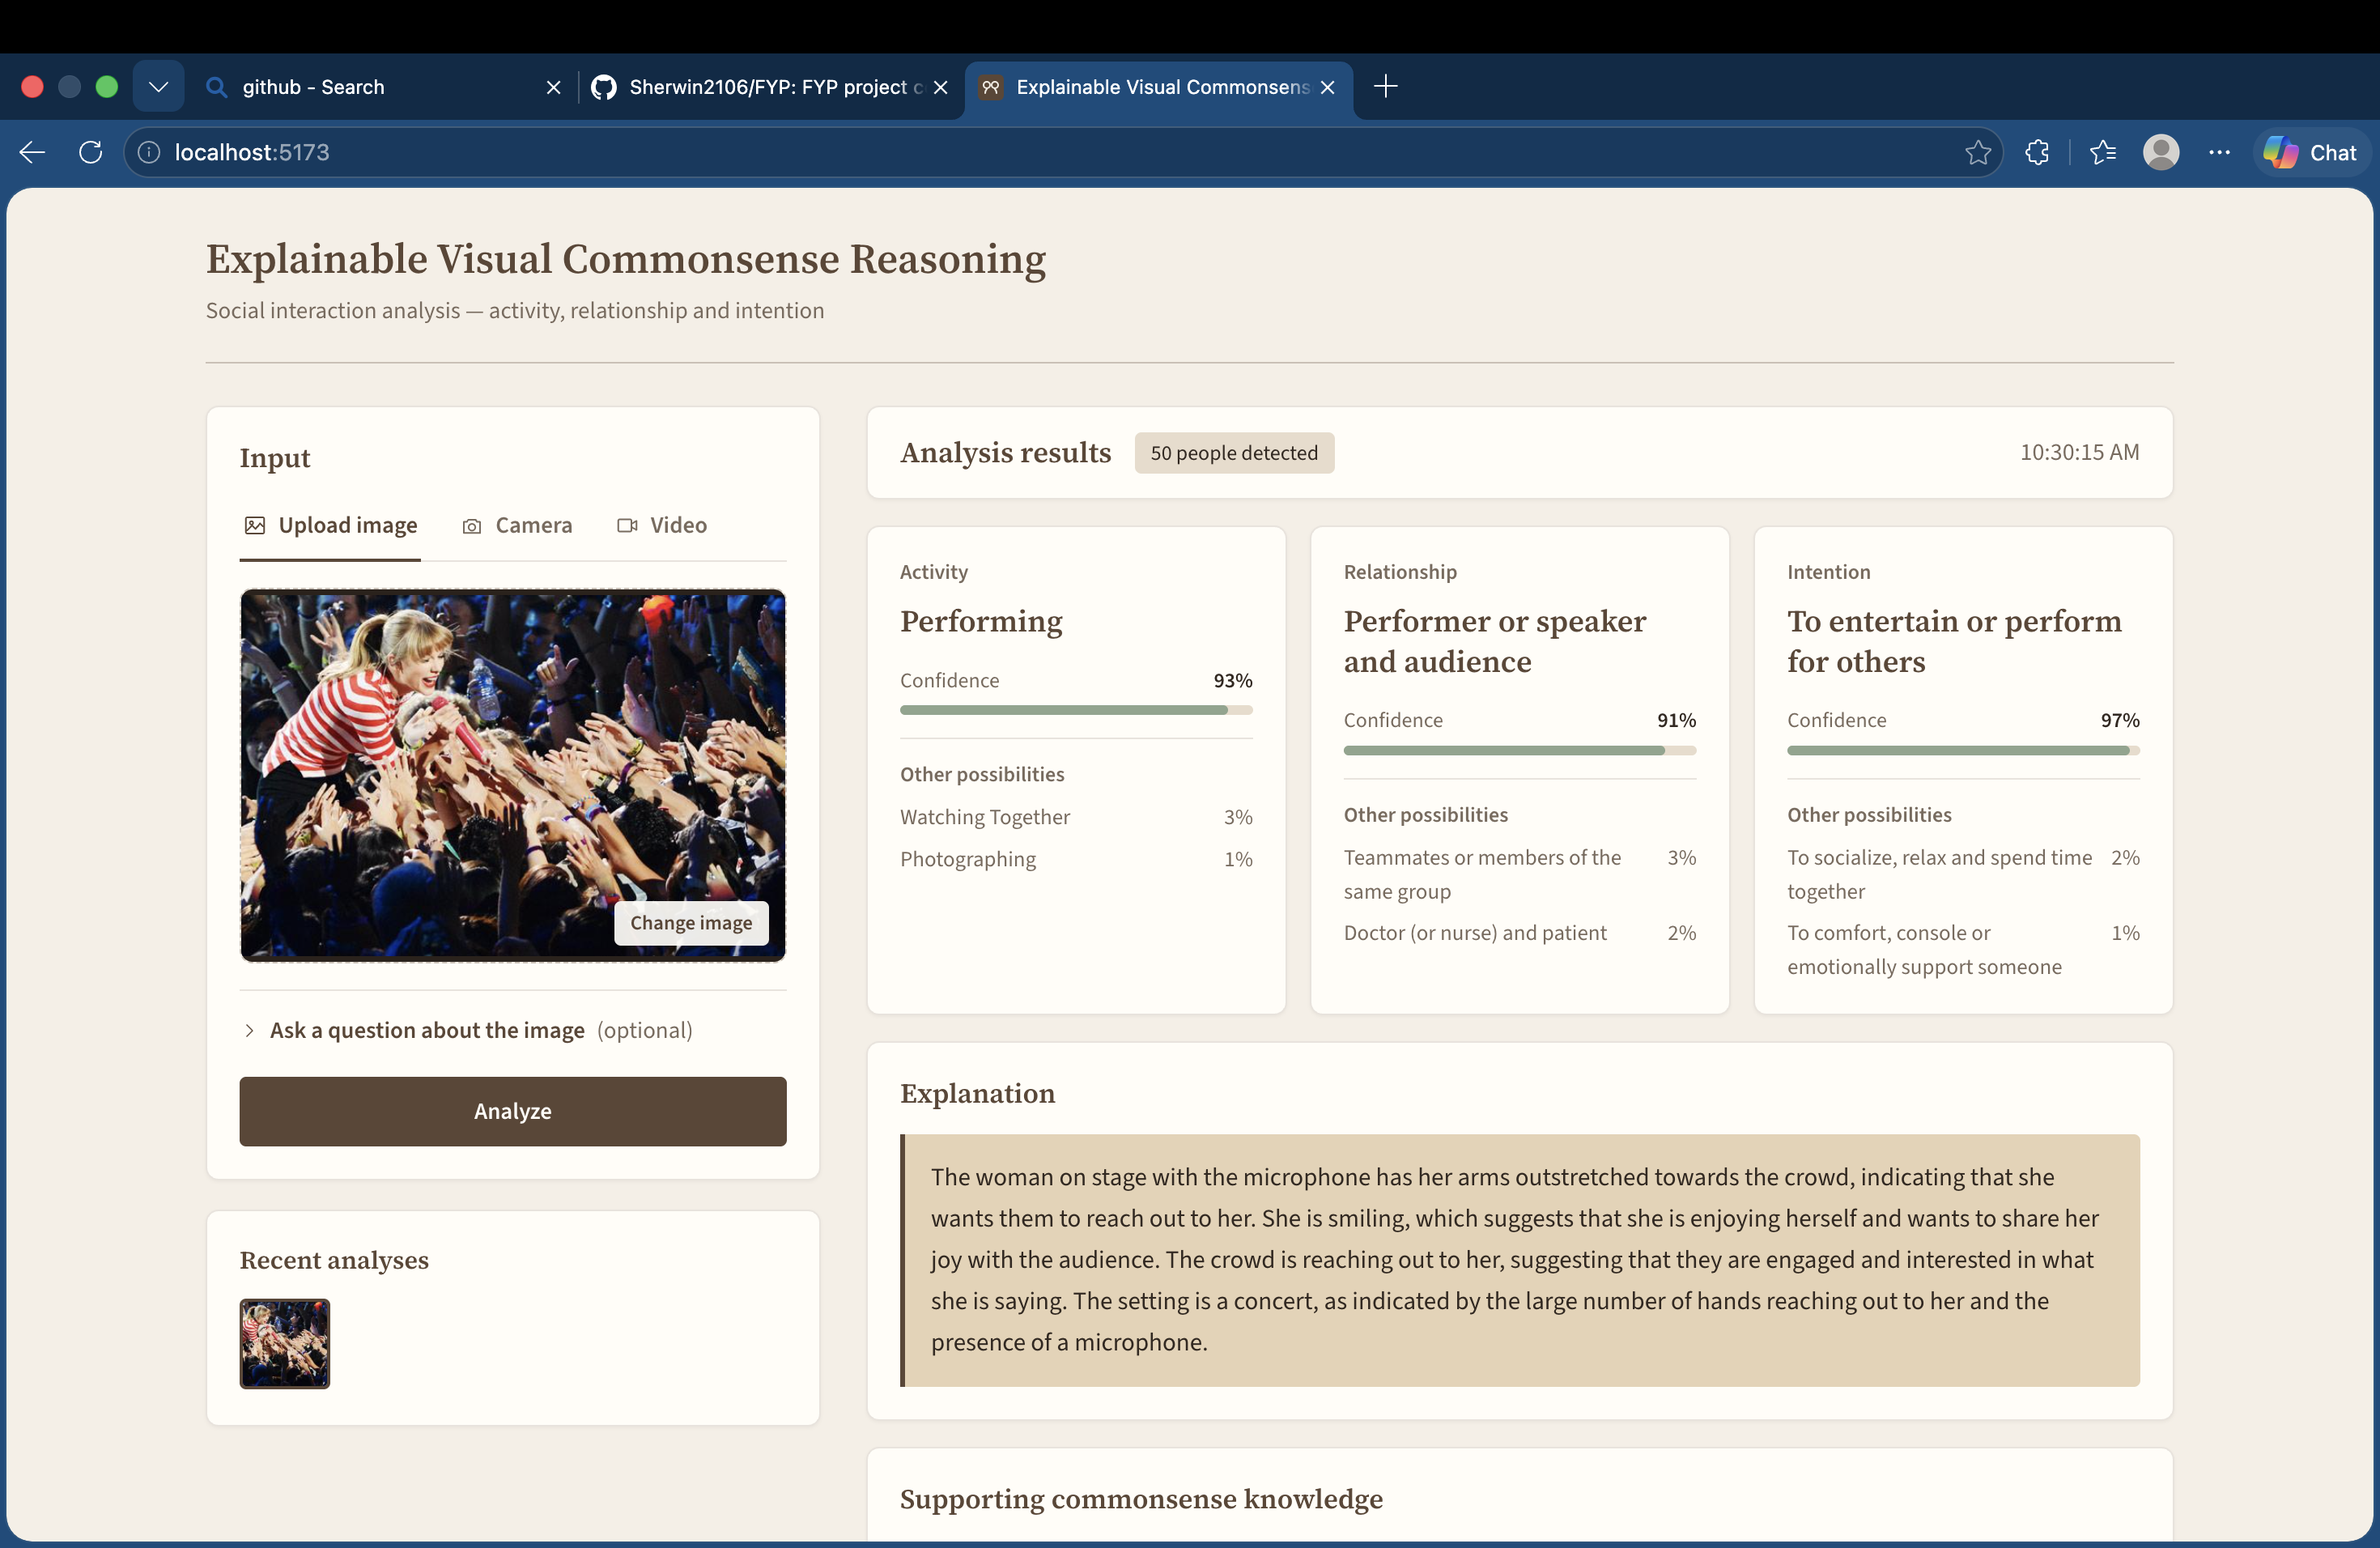
\includegraphics[width=\textwidth]{images/ui_predictions.png}
\caption{Web Interface: Predictions and Explanation for a Concert Photograph}
\label{fig:uipred}
\end{figure}

\begin{table}[h!]
\centering
\caption{Predictions for the Concert Photograph}
\label{tab:demo}
\small
\renewcommand{\arraystretch}{1.3}
\begin{tabularx}{\textwidth}{|p{2.6cm}|p{4.4cm}|c|L|}
\hline
\textbf{Task} & \textbf{Prediction} & \textbf{Conf.} & \textbf{Next Alternatives}\\ \hline
Activity & Performing & 93\% & Watching together (3\%), Photographing (1\%)\\ \hline
Relationship & Performer or speaker and audience & 91\% & Teammates (3\%), Doctor and patient (2\%)\\ \hline
Intention & To entertain or perform for others & 97\% & To socialise (2\%), To comfort someone (1\%)\\ \hline
\end{tabularx}
\end{table}

The supporting evidence and the scene description are shown in Figure~\ref{fig:uievid}. ConceptNet links the observed concepts to the predicted labels: ``concert'' and ``sing'' are closely associated with performing, a performer is typically found on a stage, and a concert is a kind of show. The VLM identified the setting as a concert, the actions as reaching out and holding up, the expressions as happy and excited, and the objects as a water bottle, a microphone and hands. The number of people reached the system's upper limit of 50, since the crowd is larger than that.

\begin{figure}[H]
\centering
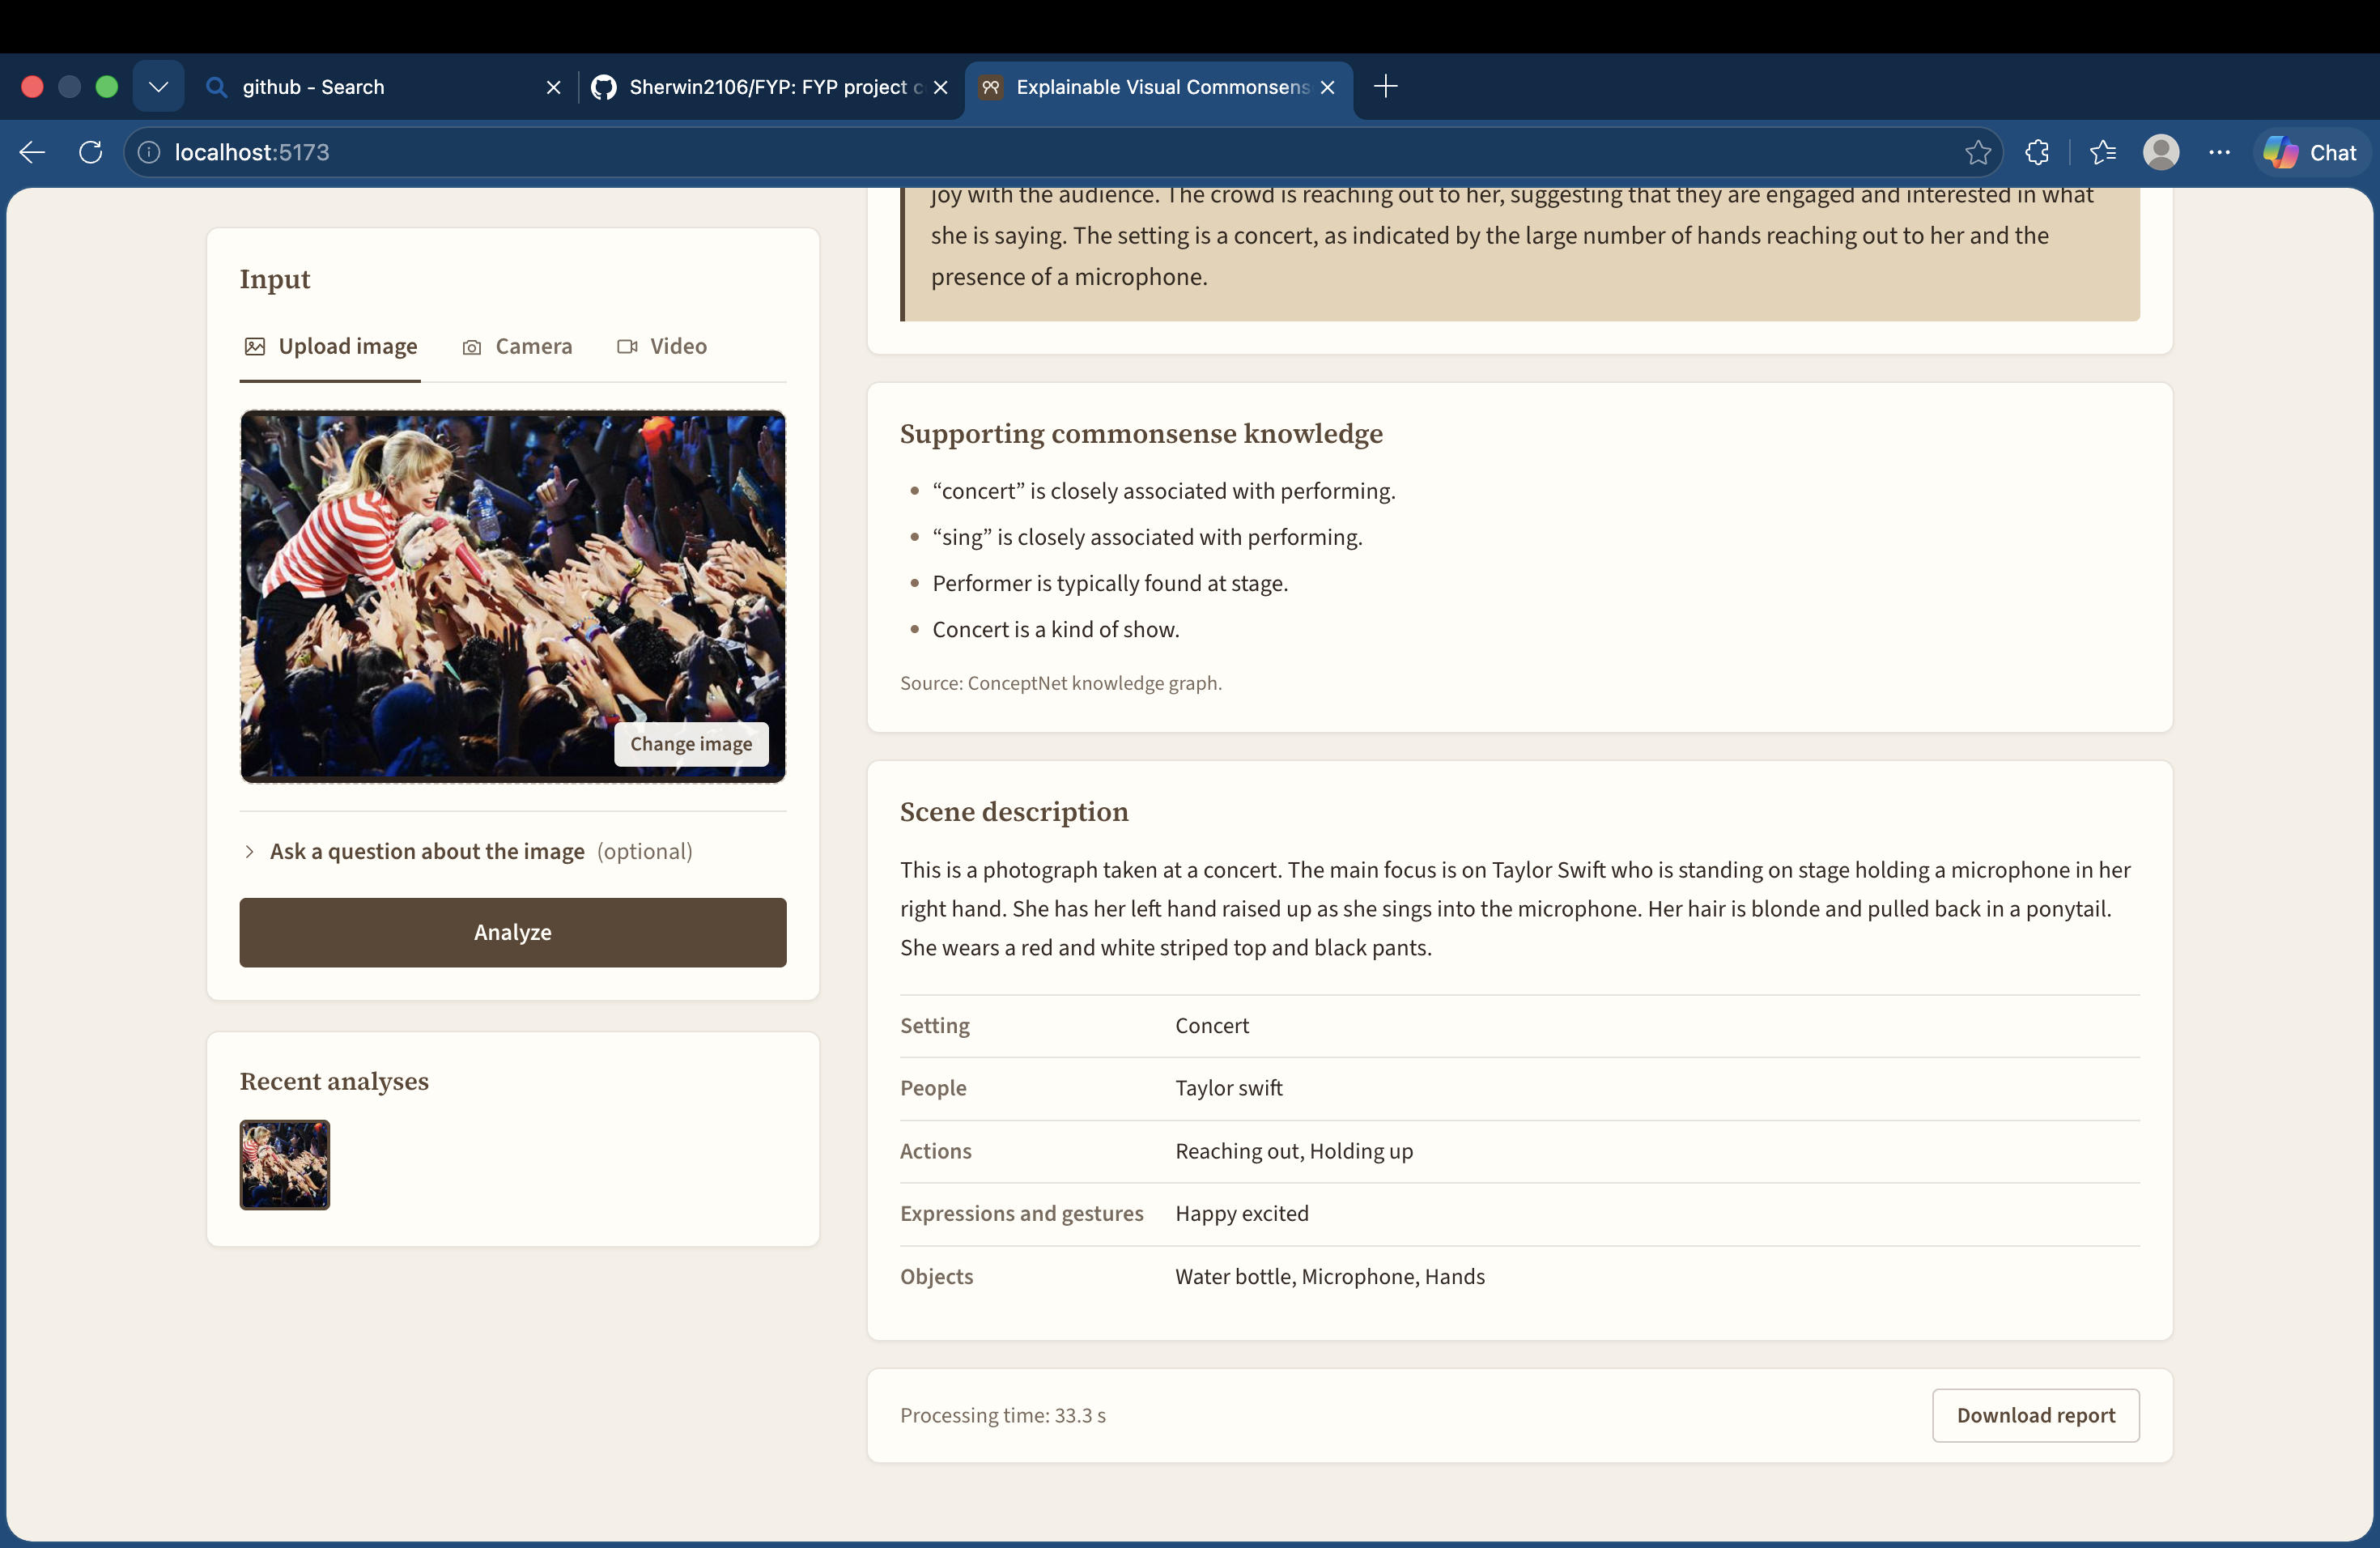
\includegraphics[width=\textwidth]{images/ui_evidence.jpg}
\caption{Web Interface: Supporting ConceptNet Knowledge and Scene Description}
\label{fig:uievid}
\end{figure}

The complete analysis of the concert photograph took 33.3 seconds on an Apple Silicon MacBook using the MPS backend. Most of this time is spent in the VLM: for a scene with two or more people and no question, Algorithm~\ref{alg:vlm} makes eleven generation calls, the explanation adds one more, and the option scoring of Algorithm~\ref{alg:mcscore} adds $k$ forward passes for each of the three tasks. The preprocessing and ConceptNet stages operate on small arrays and a local database, and contribute comparatively little. The per-module timings are recorded in every \code{Phase1Result}.

\subsection{Discussion}
Compared with a conventional image-captioning or classification pipeline, the Phase I system reasons at three levels. At the \emph{visual} level, it identifies the people, objects, actions, gestures and setting of the scene and describes them in a caption. At the \emph{commonsense} level, it links these observations to ConceptNet relations and label-support paths. At the \emph{decision} level, it fuses the VLM probabilities, the commonsense support and the draft match into a single prediction. The final prediction is therefore not a single sentence from the VLM: it retains the intermediate visual concepts, commonsense facts, component probabilities, alternatives and evidence that the explainability phase requires. Table~\ref{tab:status} summarises the status of each Phase I module.

\begin{table}[h!]
\centering
\caption{Phase I Implementation Status}
\label{tab:status}
\small
\renewcommand{\arraystretch}{1.3}
\begin{tabularx}{\textwidth}{|p{4cm}|p{2.2cm}|L|}
\hline
\textbf{Module} & \textbf{Status} & \textbf{Implemented Result}\\ \hline
Input and Preprocessing & Completed & Image/video/live input, quality checks, enhancement, resizing, normalisation and frame sampling\\ \hline
Small Vision-Language Model & Completed & SmolVLM integration, visual concept extraction, draft reasoning, deterministic generation and option scoring\\ \hline
Fine-tuning (offline) & Completed & LoRA fine-tuning on VCR for 20 epochs; epoch 11 selected; \QtoAR{} on held-out test questions raised from 15.3\% to 32.7\%\\ \hline
ConceptNet Commonsense Enrichment & Completed & Concept extraction, ConceptNet lookup, relevance filtering, label support, evidence and ambiguity resolution\\ \hline
Social Interaction Reasoning & Completed & Context fusion, activity/relationship/intention inference, log-linear fusion, confidence, alternatives and explanation generation\\ \hline
Explanation verification and dashboard & Phase II & Planned for the next phase\\ \hline
\end{tabularx}
\end{table}

\subsection{Limitations}
\begin{itemize}
\item The quantitative evaluation measures the fine-tuned VLM on VCR questions. There is not yet a labelled benchmark for the activity, relationship and intention predictions of the complete pipeline, so the end-to-end accuracy of the fused prediction has been assessed only qualitatively.
\item The fusion weights ($w_{\text{VLM}}$, $w_{\text{CN}}$, $w_{\text{draft}}$) and thresholds are set by hand; their effect has not yet been measured by an ablation study, and the calibration of the reported confidence values has not been measured.
\item The analysis of one image takes about half a minute, which is acceptable for single images but too slow for continuous real-time video.
\item The explanation is generated by the same VLM that makes the prediction, and its faithfulness has not yet been verified; this is the subject of Phase II.
\end{itemize}
 % EXPERIMENTAL RESULTS AND PERFORMANCE ANALYSIS
%-----------------------------------------
% Chapter 5 - Social Impact and Sustainability
%-----------------------------------------

\chapter{SOCIAL IMPACT AND SUSTAINABILITY}
\label{ch:impact}

\section{SOCIAL IMPACT}

Systems that interpret social interactions in images are beginning to be used in everyday tools, and making such systems explainable and lightweight has several positive applications. For people who are blind or have low vision, a description that goes beyond listing objects -- ``a performer is entertaining an audience'', ``two people appear to be arguing'' -- conveys the social meaning of a scene. Because the system runs on modest hardware, it can be deployed on personal devices without sending images to a remote server. Showing the cues behind an interpretation (gestures, expressions, posture and setting) can also support people who find non-verbal cues hard to read, and can be used in training material that teaches how such cues are interpreted.

Social and service robots need to recognise whether people are busy, in conversation or seeking help before approaching them; an inspectable reasoning chain helps developers check that such decisions are made for the right reasons. More generally, every prediction of the system comes with its evidence, its alternatives and a confidence value, and ambiguous cases are flagged. Users can see when the system is uncertain and why it reached a conclusion, which supports appropriate rather than blind trust in AI.

\subsection{Ethical Considerations}

Inferring relationships and intentions from images is sensitive, and the project recognises the following risks.
\begin{itemize}
\item \textbf{Privacy and identification:} Vision-language models may name recognisable people; in the demonstration of Section~\ref{sec:demo}, the scene description identifies the performer by name. Identity is not needed for the social-interaction task. Prompts and output filtering should prevent the system from naming individuals, and face blurring can be applied before results are stored.
\item \textbf{Surveillance misuse:} Automatic inference of relationships and intentions could be misused to monitor people without consent. The system is intended for assistive and research use with consenting users, and processes images locally without retaining them by default.
\item \textbf{Bias and stereotyping:} VCR is built from movie scenes, and pre-trained VLMs reflect their training data; such sources can encode stereotypes about who is a ``doctor'' or a ``patient'', or about gender and age roles. Biased performance across demographic groups has been documented in commercial vision systems~\cite{buolamwini2018gender}. The visible evidence and alternatives produced by this system make such biases easier to detect, and a demographic audit of the predictions is planned.
\item \textbf{Over-reliance:} A confident but wrong inference about intention can mislead. The ambiguity flag and the alternatives are shown so that users treat the output as an interpretation, not a fact.
\end{itemize}

\section{SUSTAINABILITY}

The design choices of the project reduce the computational and environmental cost of the system~\cite{strubell2019energy}. The 2.2-billion-parameter SmolVLM is far smaller than the large multimodal models commonly used for visual reasoning, so inference runs on a laptop GPU, Apple-silicon MPS or a CPU instead of a data-centre accelerator. LoRA trains only the low-rank adapters while the vision encoder, the connector and the language-model weights remain frozen; the complete training run was 1,500 optimiser steps on a single laboratory GPU. The selected adapter is merged into the base weights at load time, so the fine-tuned model costs no more to run than the base model.

Sustainability is further improved by reuse and offline operation. Commonsense knowledge comes from an existing knowledge graph queried from a local database, and the label space is a configuration file, so new labels can be added without retraining the model. The local ConceptNet database and local model make the system usable without a network connection, which reduces both data transfer and dependence on paid cloud services. For video, frame sampling skips blurry frames and frames that repeat the previous scene, so the model analyses only frames that carry new information.

\subsection{Alignment with the Sustainable Development Goals}

The project contributes to the following United Nations Sustainable Development Goals:
\begin{itemize}
\item \textbf{SDG 3 -- Good Health and Well-being:} assistive scene understanding for people with visual impairment and support for social-cue learning.
\item \textbf{SDG 9 -- Industry, Innovation and Infrastructure:} affordable, explainable AI that runs on commodity hardware.
\item \textbf{SDG 10 -- Reduced Inequalities:} lower hardware requirements widen access to multimodal AI, and transparent evidence makes biased predictions easier to find and correct.
\end{itemize}
 % SOCIAL IMPACT AND SUSTAINABILITY
\chapter{CONCLUSION AND FUTURE WORK}
\label{ch:conclusion}

In conclusion, Phase I of the project has produced a complete, tested prediction pipeline for explainable visual commonsense reasoning about social interactions. The system accepts image, video and live-camera input, standardises it with OpenCV, performs visual understanding and language reasoning with SmolVLM, enriches the detected concepts with ConceptNet, and fuses the resulting evidence in a configurable social-interaction reasoning module.

SmolVLM was fine-tuned on the VCR dataset with LoRA for 20 epochs, and the adapter from epoch 11 was selected on a held-out selection set. On separate held-out test questions it improves accuracy over the base model from 44.7\% to 58.7\% for \QtoA, from 41.3\% to 57.7\% for \QAtoR{} and from 15.3\% to 32.7\% for \QtoAR.

The main output of Phase I is a structured prediction of the activity, relationship and intention, accompanied by confidence values, alternatives, evidence and a textual explanation. The modules are connected through a reusable \code{Phase1Pipeline}, the FastAPI--React interface demonstrates the complete flow, and all 23 automated tests pass. Phase I objectives 1--10 of Section~\ref{sec:objectives} have therefore been met, and the implementation provides a tested foundation for the second phase.

As future work, Phase II will extend the system from prediction to verified explanation. Grad-CAM maps over the SmolVLM vision encoder will form a visual explanation path, and the concepts cited in the generated explanation will form an independent textual path. The Jaccard-based cross-modal consistency between the two concept sets (Equation~\ref{eq:cmc}) will be measured, faithfulness will be evaluated with the Insertion--Deletion metric and the Pointing Game, and the input frame, the predicted interaction, the three labels, the explanations and the consistency score will be presented in an explainability dashboard.

In addition, the following improvements are planned:
\begin{itemize}
\item a labelled evaluation set for the activity, relationship and intention predictions of the full pipeline, together with an ablation study of the fusion weights and of each evidence source;
\item measurement and improvement of confidence calibration;
\item a larger VCR test set and training on more VCR questions;
\item faster inference by batching the VLM prompts, to approach real-time video analysis;
\item privacy safeguards that prevent the naming of individuals, and an audit of the predictions across demographic groups.
\end{itemize}
 % CONCLUSION AND FUTURE WORK

\addtotoc{REFERENCES}
\begin{thebibliography}{99}

\bibitem{zellers2019vcr}
R.~Zellers, Y.~Bisk, A.~Farhadi, and Y.~Choi, ``From recognition to cognition: Visual commonsense reasoning,'' in \textit{Proc. IEEE/CVF Conf. on Computer Vision and Pattern Recognition (CVPR)}, 2019.

\bibitem{lin2019tabvcr}
K.~Lin \textit{et al.}, ``TAB-VCR: Tags and attributes based VCR baselines,'' in \textit{Advances in Neural Information Processing Systems (NeurIPS)}, 2019.

\bibitem{yu2019hgl}
W.~Yu \textit{et al.}, ``Heterogeneous graph learning for visual commonsense reasoning,'' in \textit{Advances in Neural Information Processing Systems (NeurIPS)}, 2019.

\bibitem{park2020visualcomet}
J.~S.~Park, C.~Bhagavatula, R.~Mottaghi, A.~Farhadi, and Y.~Choi, ``VisualCOMET: Reasoning about the dynamic context of a still image,'' in \textit{European Conf. on Computer Vision (ECCV)}, 2020.

\bibitem{lu2019vilbert}
J.~Lu, D.~Batra, D.~Parikh, and S.~Lee, ``ViLBERT: Pretraining task-agnostic visiolinguistic representations for vision-and-language tasks,'' in \textit{Advances in Neural Information Processing Systems (NeurIPS)}, 2019.

\bibitem{su2020vlbert}
W.~Su \textit{et al.}, ``VL-BERT: Pre-training of generic visual-linguistic representations,'' in \textit{Int. Conf. on Learning Representations (ICLR)}, 2020.

\bibitem{chen2020uniter}
Y.-C.~Chen \textit{et al.}, ``UNITER: UNiversal image-TExt representation learning,'' in \textit{European Conf. on Computer Vision (ECCV)}, 2020.

\bibitem{zellers2021merlot}
R.~Zellers \textit{et al.}, ``MERLOT: Multimodal neural script knowledge models,'' in \textit{Advances in Neural Information Processing Systems (NeurIPS)}, 2021.

\bibitem{radford2021clip}
A.~Radford \textit{et al.}, ``Learning transferable visual models from natural language supervision,'' in \textit{Int. Conf. on Machine Learning (ICML)}, 2021.

\bibitem{li2023blip2}
J.~Li, D.~Li, S.~Savarese, and S.~Hoi, ``BLIP-2: Bootstrapping language-image pre-training with frozen image encoders and large language models,'' in \textit{Int. Conf. on Machine Learning (ICML)}, 2023.

\bibitem{liu2023llava}
H.~Liu, C.~Li, Q.~Wu, and Y.~J.~Lee, ``Visual instruction tuning,'' in \textit{Advances in Neural Information Processing Systems (NeurIPS)}, 2023.

\bibitem{marafioti2025smolvlm}
A.~Marafioti \textit{et al.}, ``SmolVLM: Redefining small and efficient multimodal models,'' \textit{arXiv preprint}, 2025.

\bibitem{zhai2023siglip}
X.~Zhai, B.~Mustafa, A.~Kolesnikov, and L.~Beyer, ``Sigmoid loss for language image pre-training,'' in \textit{Proc. IEEE/CVF Int. Conf. on Computer Vision (ICCV)}, 2023.

\bibitem{speer2017conceptnet}
R.~Speer, J.~Chin, and C.~Havasi, ``ConceptNet 5.5: An open multilingual graph of general knowledge,'' in \textit{Proc. AAAI Conf. on Artificial Intelligence}, 2017.

\bibitem{marino2019okvqa}
K.~Marino, M.~Rastegari, A.~Farhadi, and R.~Mottaghi, ``OK-VQA: A visual question answering benchmark requiring external knowledge,'' in \textit{Proc. IEEE/CVF Conf. on Computer Vision and Pattern Recognition (CVPR)}, 2019.

\bibitem{marino2021krisp}
K.~Marino, X.~Chen, D.~Parikh, A.~Gupta, and M.~Rohrbach, ``KRISP: Integrating implicit and symbolic knowledge for open-domain knowledge-based VQA,'' in \textit{Proc. IEEE/CVF Conf. on Computer Vision and Pattern Recognition (CVPR)}, 2021.

\bibitem{sun2017domain}
Q.~Sun, B.~Schiele, and M.~Fritz, ``A domain based approach to social relation recognition,'' in \textit{Proc. IEEE Conf. on Computer Vision and Pattern Recognition (CVPR)}, 2017.

\bibitem{li2017dualglance}
J.~Li, Y.~Wong, Q.~Zhao, and M.~S.~Kankanhalli, ``Dual-glance model for deciphering social relationships,'' in \textit{Proc. IEEE Int. Conf. on Computer Vision (ICCV)}, 2017.

\bibitem{hu2022lora}
E.~J.~Hu \textit{et al.}, ``LoRA: Low-rank adaptation of large language models,'' in \textit{Int. Conf. on Learning Representations (ICLR)}, 2022.

\bibitem{dettmers2023qlora}
T.~Dettmers, A.~Pagnoni, A.~Holtzman, and L.~Zettlemoyer, ``QLoRA: Efficient finetuning of quantized LLMs,'' in \textit{Advances in Neural Information Processing Systems (NeurIPS)}, 2023.

\bibitem{selvaraju2017gradcam}
R.~R.~Selvaraju \textit{et al.}, ``Grad-CAM: Visual explanations from deep networks via gradient-based localization,'' in \textit{Proc. IEEE Int. Conf. on Computer Vision (ICCV)}, 2017.

\bibitem{petsiuk2018rise}
V.~Petsiuk, A.~Das, and K.~Saenko, ``RISE: Randomized input sampling for explanation of black-box models,'' in \textit{British Machine Vision Conf. (BMVC)}, 2018.

\bibitem{zhang2018excitation}
J.~Zhang, S.~A.~Bargal, Z.~Lin, J.~Brandt, X.~Shen, and S.~Sclaroff, ``Top-down neural attention by excitation backprop,'' \textit{Int. J. of Computer Vision}, vol.~126, pp.~1084--1102, 2018.

\bibitem{kayser2021evil}
M.~Kayser \textit{et al.}, ``e-ViL: A dataset and benchmark for natural language explanations in vision-language tasks,'' in \textit{Proc. IEEE/CVF Int. Conf. on Computer Vision (ICCV)}, 2021.

\bibitem{zhang2024crossmodal}
Zhang \textit{et al.}, ``Cross-modal consistency in multimodal large language models,'' 2024.

\bibitem{parcalabescu2025faithfulness}
L.~Parcalabescu and A.~Frank, ``Faithfulness of vision-language explanations,'' 2024--2025.

\bibitem{bradski2000opencv}
G.~Bradski, ``The OpenCV library,'' \textit{Dr. Dobb's Journal of Software Tools}, 2000.

\bibitem{zuiderveld1994clahe}
K.~Zuiderveld, ``Contrast limited adaptive histogram equalization,'' in \textit{Graphics Gems IV}, P.~S.~Heckbert, Ed. Academic Press, 1994, pp.~474--485.

\bibitem{wolf2020transformers}
T.~Wolf \textit{et al.}, ``Transformers: State-of-the-art natural language processing,'' in \textit{Proc. 2020 Conf. on Empirical Methods in Natural Language Processing: System Demonstrations}, 2020.

\bibitem{paszke2019pytorch}
A.~Paszke \textit{et al.}, ``PyTorch: An imperative style, high-performance deep learning library,'' in \textit{Advances in Neural Information Processing Systems (NeurIPS)}, 2019.

\bibitem{rohrbach2017lsmdc}
A.~Rohrbach \textit{et al.}, ``Movie description,'' \textit{Int. J. of Computer Vision}, vol.~123, pp.~94--120, 2017.

\bibitem{buolamwini2018gender}
J.~Buolamwini and T.~Gebru, ``Gender shades: Intersectional accuracy disparities in commercial gender classification,'' in \textit{Proc. Conf. on Fairness, Accountability and Transparency}, PMLR~81, 2018.

\bibitem{strubell2019energy}
E.~Strubell, A.~Ganesh, and A.~McCallum, ``Energy and policy considerations for deep learning in NLP,'' in \textit{Proc. 57th Annual Meeting of the Association for Computational Linguistics (ACL)}, 2019.

\bibitem{review1}
V.~S.~G. \textit{et al.}, ``Explainable visual commonsense reasoning for social interactions -- Review Report I,'' Department of Computer Science and Engineering, Sri Sivasubramaniya Nadar College of Engineering, 2026.

\end{thebibliography}

%% ----------------------------------------------------------------
%% Appendices (optional)
\appendix
% Appendices (optional)

\chapter{CONFIGURATION PARAMETERS}
\label{app:config}

Table~\ref{tab:params} lists the main parameters of the Phase I pipeline, set in \path{configs/default.yaml} unless stated otherwise.

\begin{table}[h!]
\centering
\caption{Main Configuration Parameters of the Phase I Pipeline}
\label{tab:params}
\small
\renewcommand{\arraystretch}{1.3}
\begin{tabularx}{\textwidth}{|p{2.8cm}|p{5.4cm}|L|}
\hline
\textbf{Module} & \textbf{Parameter} & \textbf{Value}\\ \hline
Preprocessing & Low-light trigger & brightness $< 60$ or contrast $< 25$\\ \hline
              & Enhancement & CLAHE on L channel, gamma 0.8\\ \hline
              & Blur threshold (Laplacian variance) & $< 60$\\ \hline
              & Normalisation $\mu$, $\sigma$ & (0.5, 0.5, 0.5), (0.5, 0.5, 0.5)\\ \hline
              & Video key moments (web interface) & up to 7\\ \hline
VLM           & Model & \path{HuggingFaceTB/SmolVLM-Instruct}\\ \hline
              & Decoding & greedy, repetition penalty\\ \hline
              & Fine-tuned model & \path{configs/finetuned.yaml} (epoch-11 adapter, merged)\\ \hline
ConceptNet    & Term salience & action 1.0, gesture 0.9, role 0.9, object 0.7, setting 0.6, caption 0.5\\ \hline
              & Terms kept & top 20\\ \hline
              & Facts kept & top 6 per term, top 40 overall\\ \hline
              & Back-off penalty & salience $\times 0.5$\\ \hline
              & Contradiction penalty & $-0.5$\\ \hline
Reasoning     & Fusion weights & $w_{\text{VLM}} = 1.0$, $w_{\text{CN}} = 0.5$, $w_{\text{draft}} = 1.0$\\ \hline
              & Commonsense temperature $T$ & 0.2\\ \hline
              & Shortlist size & 8 labels\\ \hline
              & Ambiguity margin & 0.15\\ \hline
              & Maximum people count & 50\\ \hline
\end{tabularx}
\end{table}

\chapter{API ENDPOINTS}
\label{app:api}

Table~\ref{tab:api} lists the FastAPI endpoints implemented for the Phase I demonstration.

\begin{table}[h!]
\centering
\caption{FastAPI Endpoints Implemented for the Phase I Demonstration}
\label{tab:api}
\small
\renewcommand{\arraystretch}{1.3}
\begin{tabularx}{\textwidth}{|p{5.4cm}|L|}
\hline
\textbf{Endpoint} & \textbf{Purpose}\\ \hline
\code{GET /api/health} & Reports backend, model and ConceptNet status.\\ \hline
\code{POST /api/analyze} & Accepts an image and an optional question and choices, and creates an analysis job.\\ \hline
\code{POST /api/analyze-video} & Accepts a video, selects key moments and analyses each of them.\\ \hline
\code{GET /api/jobs/\{job\_id\}} & Returns the job status, the active module, the completed stages and the final result.\\ \hline
\end{tabularx}
\end{table}


\end{spacing}
\end{document}
